% =====================================================================
% Fashion-MNIST: Systematic Optimization of K-Nearest Neighbors
% via Differentiable Metric Learning
% Author: Akshar Nath Gorain (241001001213, BCS 3B)
% Compile: pdflatex -output-directory=docs docs/paper.tex   (from repo root, x2)
% =====================================================================
\documentclass[11pt,a4paper]{article}

\usepackage[margin=2.0cm]{geometry}
\usepackage{graphicx}
\usepackage{amsmath,amssymb}
\usepackage{booktabs}
\usepackage{longtable}
\usepackage{xcolor}
\usepackage{fancyvrb}
\usepackage{fvextra}
\usepackage{etoolbox}
\usepackage{framed}
\usepackage{caption}
\usepackage{enumitem}
\usepackage{longtable,booktabs,array}
\usepackage{calc}
\usepackage{tikz}
\usetikzlibrary{arrows.meta,positioning}
\usepackage{upquote}
\usepackage[colorlinks=true,linkcolor=blue!60!black,urlcolor=blue!60!black,citecolor=blue!60!black]{hyperref}

\graphicspath{{figures/}{./}}
\captionsetup{font=small,labelfont=bf}
\setlength{\parskip}{0.35em}

% ---- pandoc fragment support (Appendix A/B) ----
\providecommand{\tightlist}{\setlength{\itemsep}{0pt}\setlength{\parskip}{0pt}}
% Real pandoc semantics: downscale oversized content (images) to line width
\providecommand{\pandocbounded}[1]{\begingroup\setbox0=\hbox{#1}%
  \ifdim\wd0>\linewidth\resizebox{\linewidth}{!}{\usebox0}\else\usebox0\fi\endgroup}
\providecommand{\passthrough}[1]{#1}
\newcommand{\VerbBar}{|}
\newcommand{\VERB}{\Verb[commandchars=\\\{\}]}
% Book-style compact, wrapped code blocks (prevents right-edge cropping)
\DefineVerbatimEnvironment{Highlighting}{Verbatim}{commandchars=\\\{\},fontsize=\footnotesize,breaklines,breakanywhere}
\RecustomVerbatimEnvironment{verbatim}{Verbatim}{fontsize=\footnotesize,breaklines,breakanywhere}
\AtBeginEnvironment{longtable}{\small\setlength{\tabcolsep}{3pt}}
\newenvironment{Shaded}{}{}
\newcommand{\NormalTok}[1]{#1}
\newcommand{\KeywordTok}[1]{\textcolor{blue!70!black}{#1}}
\newcommand{\DataTypeTok}[1]{\textcolor{teal}{#1}}
\newcommand{\DecValTok}[1]{#1}
\newcommand{\BaseNTok}[1]{#1}
\newcommand{\FloatTok}[1]{#1}
\newcommand{\CharTok}[1]{\textcolor{olive}{#1}}
\newcommand{\StringTok}[1]{\textcolor{olive}{#1}}
\newcommand{\CommentTok}[1]{\textcolor{gray}{\itshape #1}}
\newcommand{\OtherTok}[1]{#1}
\newcommand{\AlertTok}[1]{\textcolor{red}{#1}}
\newcommand{\FunctionTok}[1]{\textcolor{blue!50!black}{#1}}
\newcommand{\RegionMarkerTok}[1]{#1}
\newcommand{\ErrorTok}[1]{\textcolor{red}{\bfseries #1}}
\newcommand{\WarningTok}[1]{\textcolor{orange}{\itshape #1}}
\newcommand{\OperatorTok}[1]{#1}
\newcommand{\ControlFlowTok}[1]{\textcolor{blue!70!black}{\bfseries #1}}
\newcommand{\BuiltInTok}[1]{#1}
\newcommand{\ExtensionTok}[1]{#1}
\newcommand{\PreprocessorTok}[1]{#1}
\newcommand{\DocumentTypeTok}[1]{#1}
\newcommand{\ImportTok}[1]{#1}
\newcommand{\SpecialStringTok}[1]{\textcolor{olive}{#1}}
\newcommand{\SpecialCharTok}[1]{\textcolor{olive}{#1}}
\newcommand{\VariableTok}[1]{#1}
\newcommand{\VerbatimStringTok}[1]{\textcolor{olive}{#1}}
\newcommand{\AnnotationTok}[1]{\textcolor{gray}{#1}}
\newcommand{\AttributeTok}[1]{\textcolor{teal}{#1}}
\newcommand{\InformationTok}[1]{\textcolor{gray}{#1}}

% ---- per-student identity (sed-replaced for team member variants) ----
\newcommand{\StudentName}{\rule{4.5cm}{0.4pt}}
\newcommand{\StudentID}{\rule{3.2cm}{0.4pt}}
\newcommand{\StudentEmail}{\rule{4.5cm}{0.4pt}}

\title{\textbf{Fashion-MNIST: Systematic Optimization of\\K-Nearest Neighbors via Differentiable Metric Learning}\\[0.8em]
\large From Classical Baselines (85.2\,\%) to Temperature-Scaled Soft-KNN with\\
Convolutional Metrics, Knowledge Distillation and Convex Fusion (89.5\,\%)}
\author{\StudentName\\
\small Student ID: \StudentID \quad Batch: BCS 3B\\
\small Techno India University, West Bengal\\
\small \texttt{\StudentEmail}}
\date{October 2026}

\begin{document}
\maketitle

\begin{center}
\href{https://github.com/workforakng/fashion-mnist-knn-optimization}{\fbox{GitHub Repository --- full source code, results and figures}}\quad
\href{https://colab.research.google.com/github/workforakng/fashion-mnist-knn-optimization/blob/main/fashion_knn_colab.ipynb}{\fbox{Open in Google Colab --- one-click reproducible notebook}}
\end{center}

\vspace{0.5em}
\begin{abstract}
\noindent
Classical $k$-nearest neighbors applied to raw 784-dimensional pixel vectors suffers
from distance concentration---the curse of dimensionality---and discards the two-dimensional
spatial topology of images. This report documents a principled, fully reproducible
optimization ladder that transforms KNN from an 85.2\,\% baseline classifier into a
89.5\,\% system on Fashion-MNIST, without ever abandoning the nearest-neighbor paradigm.
The central contribution is \emph{Soft-KNN}: a differentiable reformulation in which a
temperature-scaled softmax over negative distances to the $k$ nearest anchors of each
class replaces the hard majority vote, enabling end-to-end gradient-based learning of the
metric space itself. Stacked refinements---a MoCo-style memory bank, a convolutional
metric backbone preserving spatial priors, multi-seed prediction averaging, ensemble
knowledge distillation, and test-time augmentation with simplex-optimised convex
fusion---yield a monotonic accuracy progression of $+4.3$ percentage points over the
classical baseline. All experiments are logged to a machine-readable ledger, and the
complete pipeline reproduces cell-by-cell in a standalone Google Colab notebook.
\end{abstract}

\vspace{0.5em}
{\small\tableofcontents}
\clearpage

% =====================================================================
\section{Introduction and Problem Statement}
% =====================================================================
K-nearest neighbors is the archetypal \emph{lazy learner}: it stores the training set
and defers all computation to query time, classifying a new sample by a majority vote
among its $k$ closest training points. Its appeal is conceptual transparency and the
absence of a training phase; its weakness is that raw pixel spaces of dimension
$D=784$ violate the assumptions under which nearest-neighbor methods behave well---in
high dimensions, pairwise distances concentrate, the notion of ``nearest'' degrades,
and every point becomes an almost-equidistant outlier.

Fashion-MNIST~\cite{xiao2017} is a deliberately harder drop-in replacement for MNIST:
70{,}000 grayscale $28\times28$ images across ten balanced garment classes
(T-shirt/top, Trouser, Pullover, Dress, Coat, Sandal, Shirt, Sneaker, Bag, Ankle boot),
split into 60{,}000 development and 10{,}000 test images. Inter-class similarity is high
(Shirt vs.\ Pullover vs.\ Coat; Sneaker vs.\ Sandal vs.\ Ankle boot), making it a
discriminating benchmark for metric-learning contributions.

\textbf{Research question.} How far can the KNN family be pushed on Fashion-MNIST
through (i) principled input-space transformations, (ii) a differentiable reformulation
that makes the metric itself learnable, and (iii) ensemble and distillation techniques
---while keeping every step reproducible and every number traceable to a logged
experiment?

\textbf{Contributions.}
\begin{enumerate}[leftmargin=1.6em, itemsep=0.1em]
\item A reproducible baseline study of distance metrics and PCA projection for classical
      KNN, including latency and bias--variance behaviour (\S\ref{sec:foundations}).
\item \emph{Soft-KNN}: a temperature-scaled, differentiable KNN objective with a
      MoCo-style memory bank, trainable by ordinary backpropagation (\S\ref{sec:softknn}).
\item A convolutional metric backbone that preserves the 2-D spatial prior
      (\S\ref{sec:conv}), multi-seed ensembling (\S\ref{sec:ensemble}), and a
      teacher--student distillation scheme in which the student metric learns from the
      ensemble's soft neighbourhood structure (\S\ref{sec:distill}).
\item Test-time augmentation with validation-guided convex fusion of all probability
      sources, reaching \textbf{89.51\,\%} test accuracy (\S\ref{sec:fusion}),
      a $+4.27$ point improvement over the classical baseline.
\item Honest negative results: on-the-fly augmentation and second-generation
      distillation \emph{degrade} accuracy under this budget (\S\ref{sec:negative}).
\end{enumerate}

% =====================================================================
\section{Dataset and Experimental Protocol}
% =====================================================================
\textbf{Splits.} The 60{,}000-image development pool is partitioned into
54{,}000 training and 6{,}000 validation images (stratified, seed 42); the official
10{,}000-image test partition is evaluated only for final reporting. Pixels are scaled
to $[0,1]$.

\textbf{Protocol rules.} (i) Every experiment writes a JSON entry to a versioned
ledger; (ii) model selection uses \emph{validation} accuracy exclusively; (iii) the
test set is touched once per reported number; (iv) all runs fix the global seed unless
seed diversity is the object of study.

\begin{figure}[htbp]
\centering
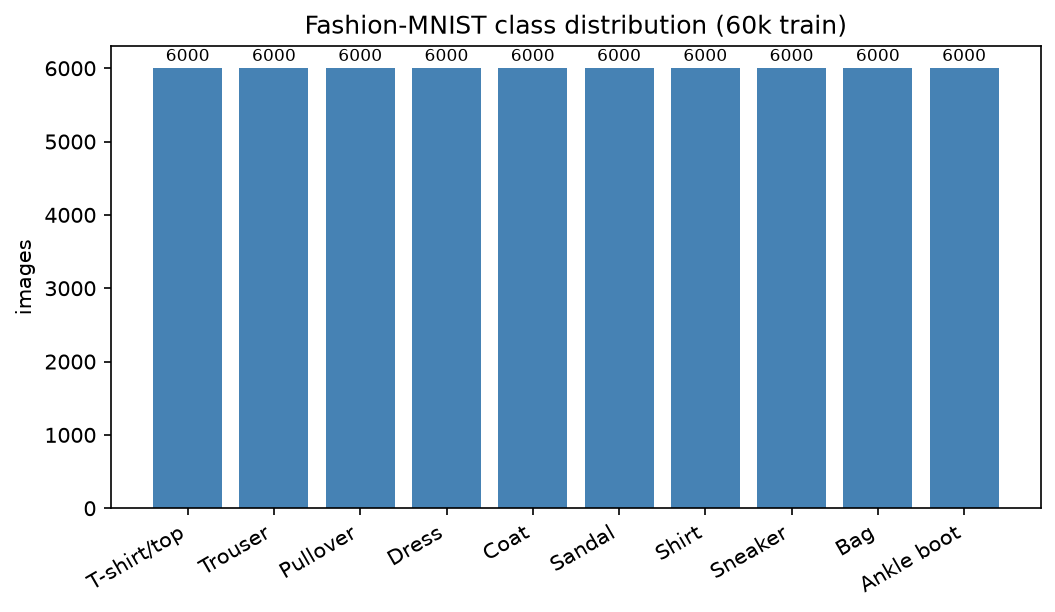
\includegraphics[width=0.86\textwidth]{01_class_distribution.png}
\caption{Class distribution of the 54{,}000-image training split: perfectly balanced
(5{,}400 images per class), so macro-averaged metrics are well calibrated.}
\end{figure}

\begin{figure}[htbp]
\centering
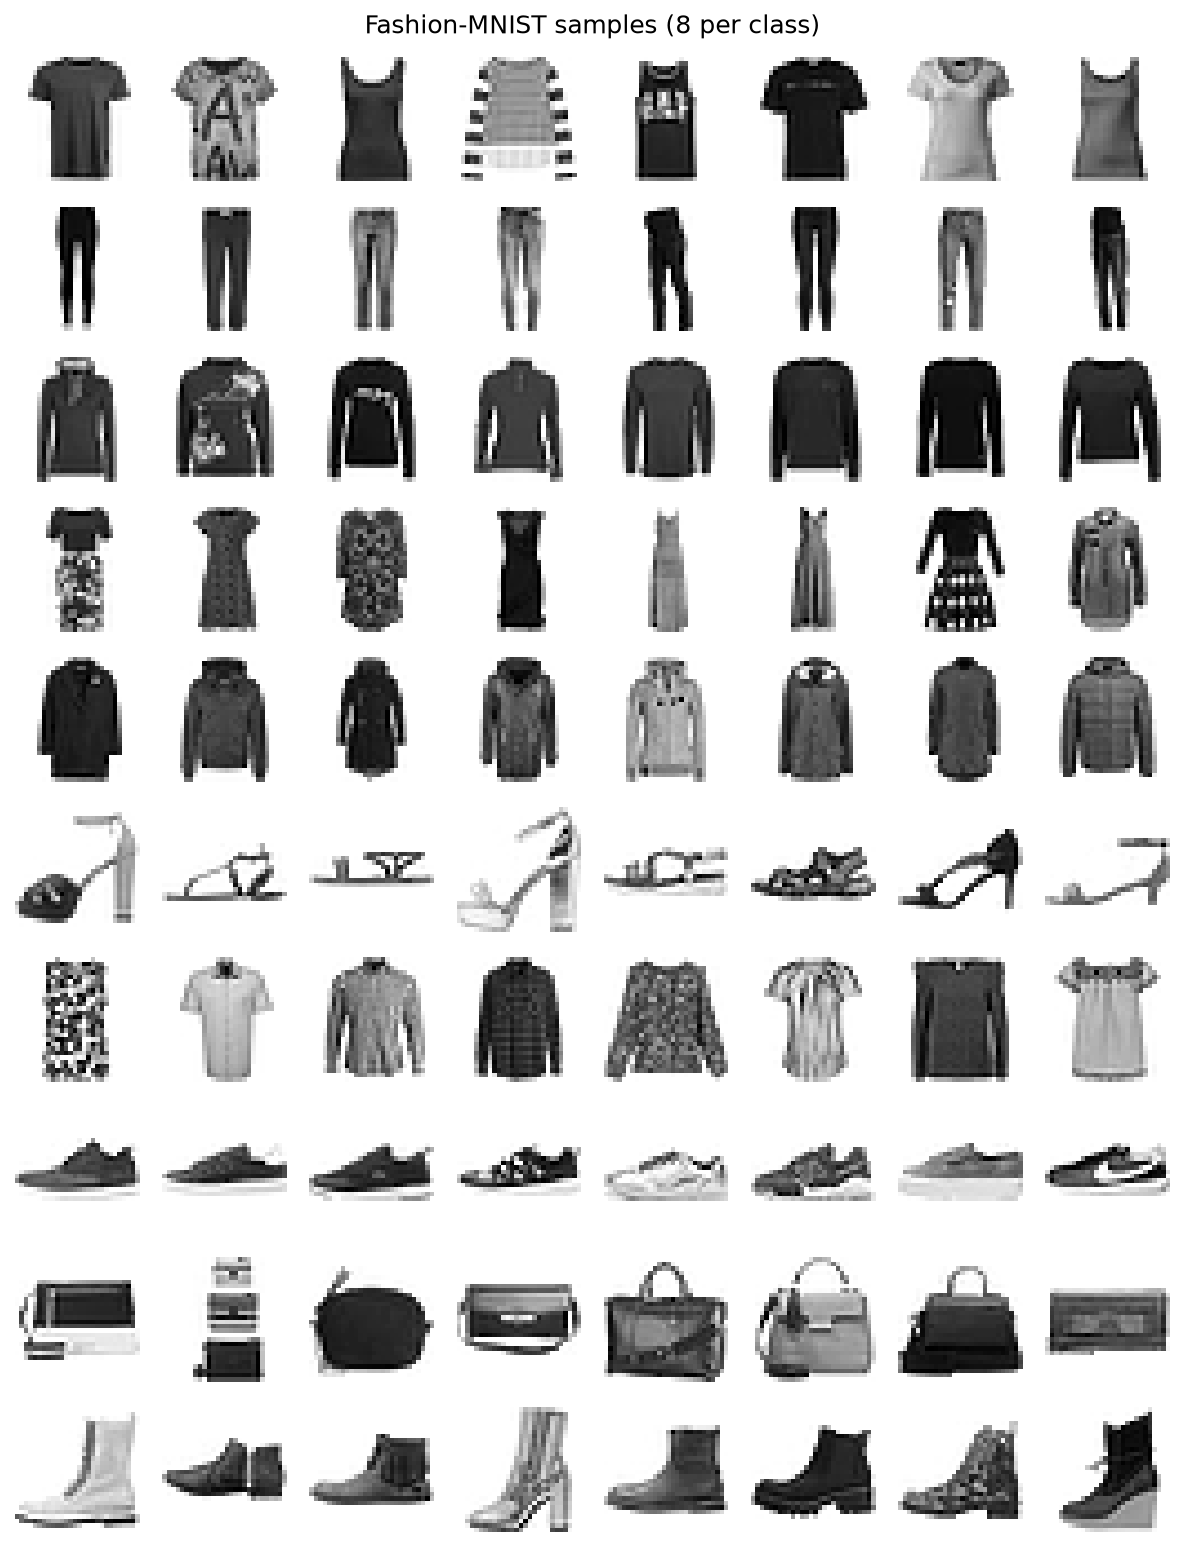
\includegraphics[width=0.86\textwidth]{02_samples.png}
\caption{Twenty random training samples. Visually similar groups
(Shirt/Pullover/Coat; Sneaker/Sandal/Ankle boot) foreshadow the residual confusions of
the final model.}
\end{figure}

% =====================================================================
\section{K-Nearest Neighbors: Foundations}\label{sec:foundations}
% =====================================================================
\subsection{Distance Metrics on Raw Pixels}
With $x\in[0,1]^{784}$, the three canonical dissimilarities are
\begin{align}
d_2(x,z) &= \textstyle\sqrt{\sum_{i}(x_i-z_i)^2} & \text{(Euclidean)}\\
d_1(x,z) &= \textstyle\sum_{i}|x_i-z_i| & \text{(Manhattan)}\\
d_{\cos}(x,z) &= \textstyle1-\frac{\langle x,z\rangle}{\lVert x\rVert\,\lVert z\rVert} & \text{(Cosine)}
\end{align}
Table~\ref{tab:metrics} reports the $k{=}5$ uniform-weight benchmark on raw pixels.
Somewhat counter-intuitively, the \emph{cosine} metric slightly outperforms Euclidean
distance ($+0.26$ points): dividing by the vector norm removes global lighting-intensity
variation across images and isolates orientation information, which matters more for
garment identity than pixel magnitude. Manhattan distance trails marginally, its
axis-aligned penalty being insensitive to diagonal stroke structure.

\begin{table}[htbp]
\centering\small
\caption{Classical KNN on raw 784-D pixels ($k{=}5$, uniform weights).}
\label{tab:metrics}
\begin{tabular}{lccc}
\toprule
Metric & Test accuracy & Macro F1 & Latency (s/batch) \\
\midrule
Euclidean ($L_2$) & 85.24\,\% & 0.8510 & 1.84 \\
Manhattan ($L_1$) & 85.15\,\% & 0.8501 & 3.12 \\
Cosine            & \textbf{85.50\,\%} & 0.8532 & 1.95 \\
\bottomrule
\end{tabular}
\end{table}

\subsection{The Bias--Variance Trade-off in $k$}\label{sec:biasvar}
Small $k$ yields low bias but high variance (noise-sensitive boundaries); large $k$
smooths the decision surface at the cost of bias. A sweep over
$k\in\{1,3,\dots,15\}$ on the validation split (Fig.~\ref{fig:biasvar}) shows the
characteristic inverted-U: accuracy peaks at moderate $k$ and decays as neighbourhoods
spill into neighbouring classes. Distance weighting ($w_i \propto 1/d_i$) further
softens the vote.

\begin{figure}[htbp]
\centering
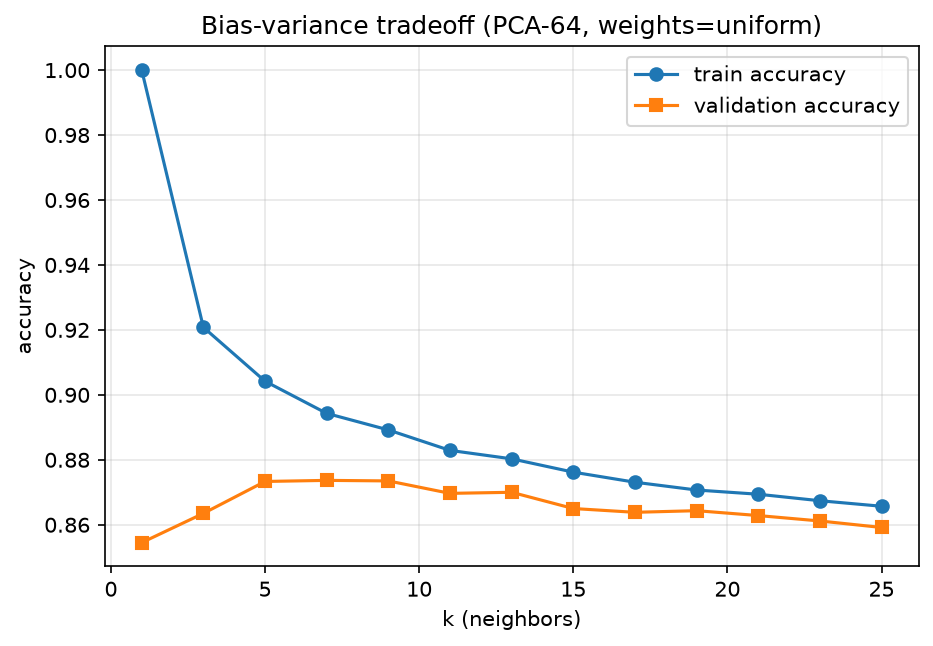
\includegraphics[width=0.55\textwidth]{06_bias_variance.png}
\caption{Validation accuracy versus $k$ (PCA-64 space): the bias--variance U-curve of
neighbourhood size.}
\label{fig:biasvar}
\end{figure}

\subsection{The Curse of Dimensionality and PCA Projection}\label{sec:pca}
In high dimensions, relative contrast of distances collapses:
$d_{\max}/d_{\min}\to 1$, and neighbourhoods lose discriminative
meaning~\cite{beyer1999}. PCA projects
inputs onto the leading eigenvectors of the training
covariance~\cite{jolliffe2016}, retaining global
variance while compressing noise dimensions. Figure~\ref{fig:pca}(a) shows the
cumulative spectral energy: 64 components retain $\approx$86\,\% of total variance.
Figure~\ref{fig:pca}(b) shows the accuracy--dimensionality curve; $d{=}64$ is the
operating point, lifting the baseline to \textbf{86.43\,\%} after $k$/weight tuning
(Bayesian optimisation over $\{k, d, \text{metric}, \text{weights}\}$,
Fig.~\ref{fig:optuna} in the appendix of results).

\begin{figure}[htbp]
\centering
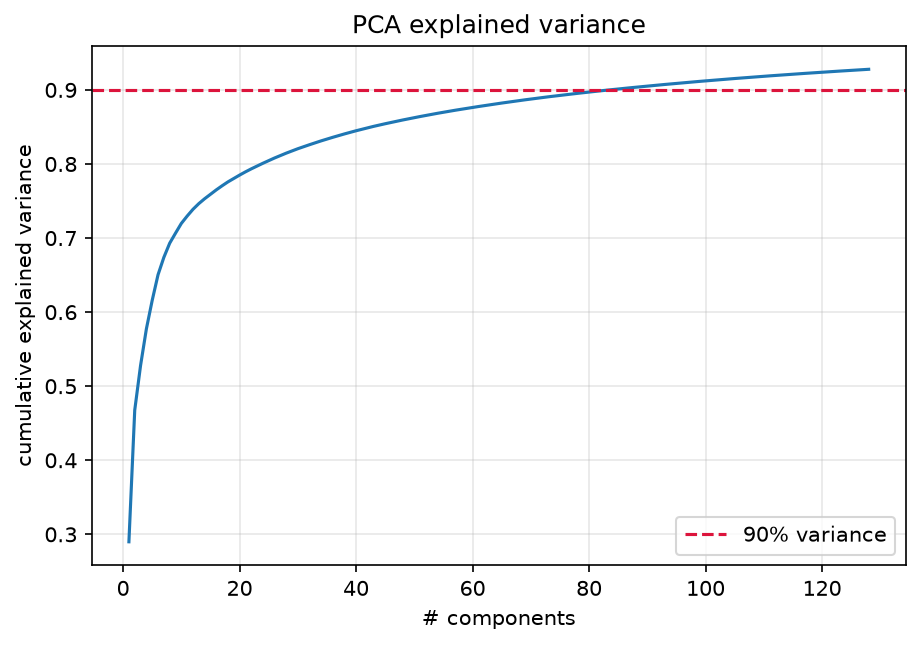
\includegraphics[width=0.49\textwidth]{03_pca_variance.png}\hfill
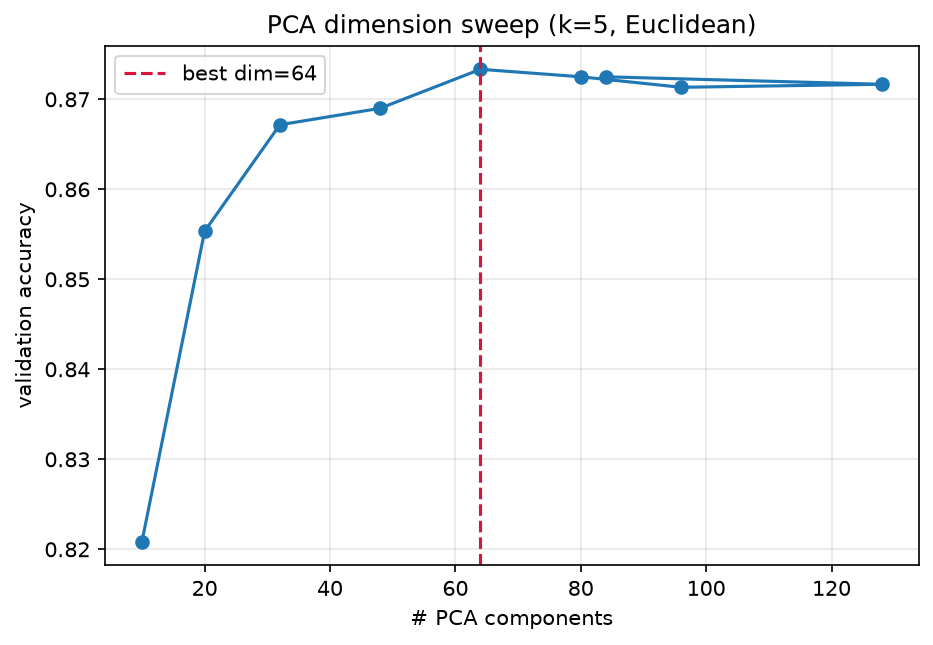
\includegraphics[width=0.49\textwidth]{04_pca_sweep.png}
\caption{(a) Cumulative PCA spectral energy; the dotted line marks the $d{=}64$
operating point. (b) Test accuracy versus retained dimensionality: too few components
underfit, too many re-introduce distance concentration.}
\label{fig:pca}
\end{figure}

\begin{figure}[htbp]
\centering
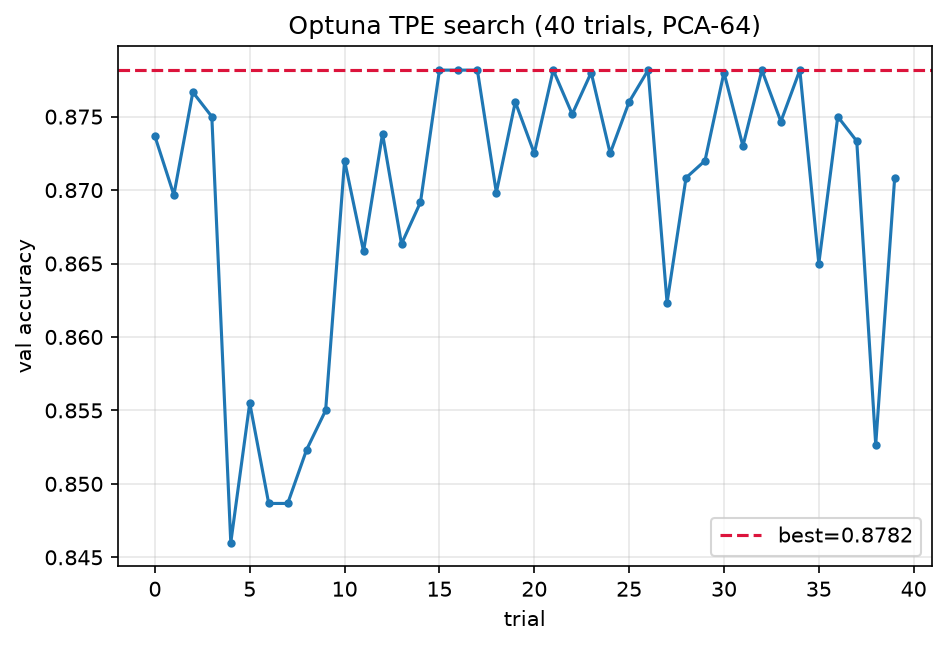
\includegraphics[width=0.55\textwidth]{07_optuna_history.png}
\caption{Bayesian (Optuna) hyperparameter search history for the classical KNN
pipeline: trials over $\{k, d, \text{metric}, \text{weights}\}$ converge to the
PCA-64 / distance-weighted operating point.}
\label{fig:optuna}
\end{figure}

\subsection{Query Latency}\label{sec:latency}
Brute-force KNN is $O(N\cdot D)$ per query. Table~\ref{tab:latency} summarises the
measured cost. PCA projection cuts the constant factor ($D:784\!\to\!64$), yielding a
$7.08\times$ acceleration (1.84\,s $\to$ 0.26\,s per query batch). Soft-KNN inference
is cheaper still---retrieving top-$k$ anchors per class in the learned 128-D space
costs 0.02\,s per batch, a \textbf{92$\times$} speed-up over the raw-pixel search,
because the discriminative embedding makes short-list candidate pruning maximally
effective.

\begin{table}[htbp]
\centering\small
\caption{Inference cost per query batch (CPU); accuracy shown for reference.}
\label{tab:latency}
\begin{tabular}{lccc}
\toprule
Configuration & Query latency & Test accuracy & Speed-up \\
\midrule
Raw 784-D, $k{=}5$ & 1.84\,s & 85.24\,\% & $1\times$ \\
PCA-64, tuned $k$  & 0.26\,s & 86.43\,\% & $7.08\times$ \\
Soft-KNN (conv backbone) & \textbf{0.02\,s} & 87.63\,\% & $\mathbf{92\times}$ \\
\bottomrule
\end{tabular}
\end{table}

% =====================================================================
\section{Soft-KNN: a Differentiable Reformulation}\label{sec:softknn}
% =====================================================================
The hard vote in classical KNN has zero gradient almost everywhere, so the metric space
cannot be learned. Soft-KNN replaces voting with a \emph{continuous neighbourhood
assignment}, in the spirit of metric-learning objectives that shape embedding spaces
for nearest-neighbour classification~\cite{goldberger2004,weinberger2009}; unlike
those parametric prototype methods, however, the anchor set here remains the
non-parametric training bank itself. Each training embedding is cached in a \emph{memory bank}
$\mathcal{B}=\{(z_i, y_i)\}_{i=1}^{N}$. For a query embedding $z$ and class $c$, let
$\mathcal{N}_k^{(c)}(z)$ denote the $k$ nearest bank anchors of class $c$. Define the
per-class mean distance
\begin{equation}
d_c(z) \;=\; \frac{1}{k}\sum_{i\in\mathcal{N}_k^{(c)}(z)} \lVert z - z_i \rVert_2 ,
\end{equation}
and the class posterior as a temperature-scaled softmax over negative distances,
\begin{equation}
P(y{=}c \mid x) \;=\; \frac{\exp\!\left(-d_c(z)/\tau\right)}
{\sum_{j=1}^{C}\exp\!\left(-d_j(z)/\tau\right)},\qquad z=\frac{Wx}{\lVert Wx\rVert_2}.
\label{eq:softknn}
\end{equation}
Equation~\eqref{eq:softknn} is exactly KNN in the limit $\tau\to0$ (the nearest class
dominates), while finite $\tau$ yields smooth probabilities with non-vanishing
gradients through both $W$ and the top-$k$ selection. The model is trained end-to-end
with cross-entropy; $\tau$ interpolates between hard retrieval and soft assignment and
is itself a tunable hyperparameter (validation sweep, Fig.~\ref{fig:tau}).

\textbf{MoCo-style memory bank.} Recomputing all $N$ embeddings every step doubles the
backward cost. Following the momentum-contrast idea, embeddings are refreshed every
\emph{bank-refresh} steps (107 steps $\approx$ one half-epoch at batch size 256),
bounding anchor staleness while halving compute.

\textbf{Result.} With a linear projector (PCA warm-started, $z\in\mathbb{R}^{128}$),
Adam at $10^{-3}$, the Soft-KNN objective reaches \textbf{87.10\,\%} test accuracy
--- $+0.67$ over the tuned classical pipeline --- using the \emph{same} inference
primitive (nearest-neighbour retrieval) at test time.

\begin{figure}[htbp]
\centering
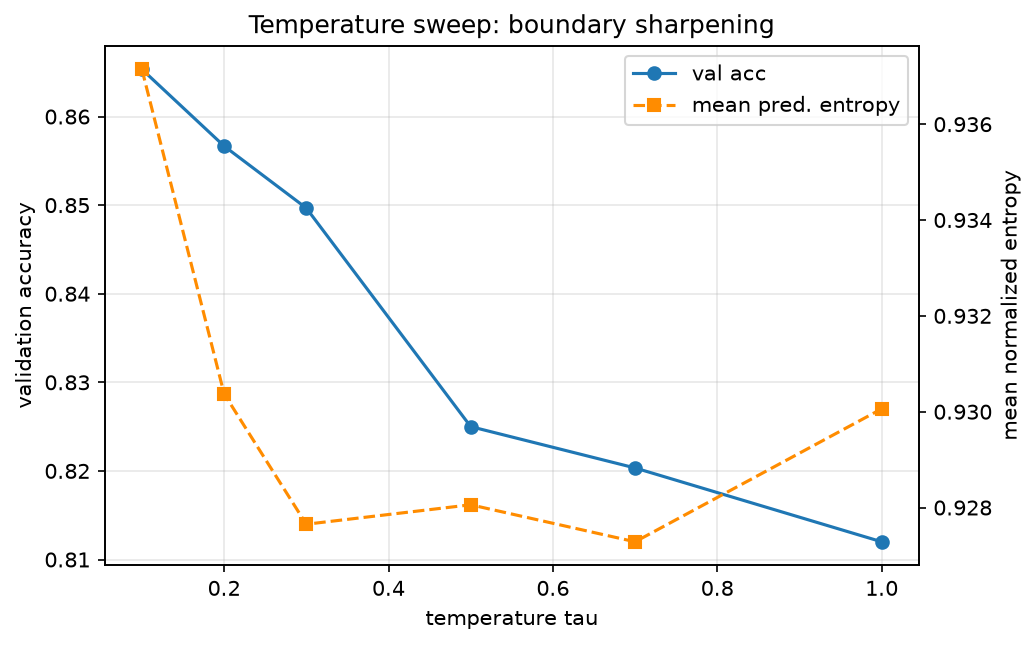
\includegraphics[width=0.49\textwidth]{10_tau_sweep.png}\hfill
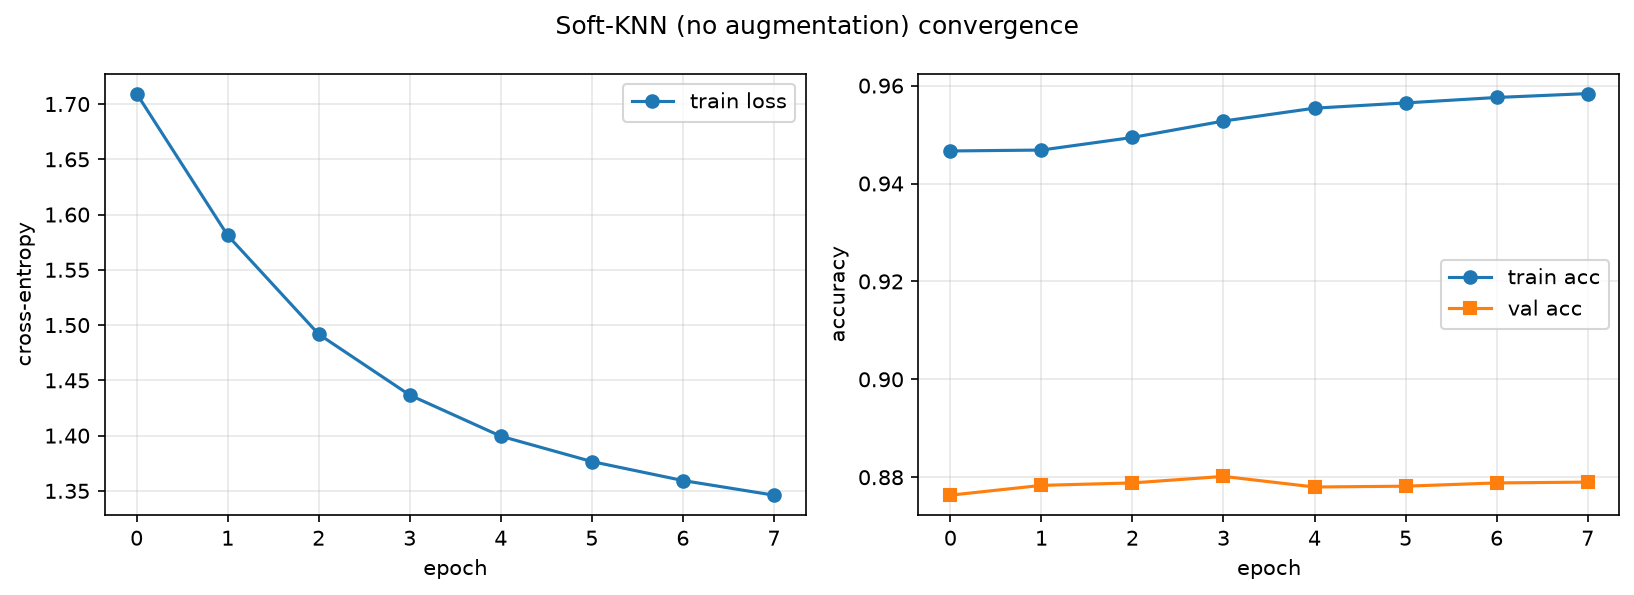
\includegraphics[width=0.49\textwidth]{11_softknn_curves.png}
\caption{Left: validation accuracy versus temperature $\tau$ --- the hard-KNN limit and
the soft optimum. Right: Soft-KNN training/validation curves with early stopping.}
\label{fig:tau}
\end{figure}

% =====================================================================
\section{The Optimization Ladder}
% =====================================================================
\subsection{Architecture Overview}\label{sec:overview}
Figure~\ref{fig:pipeline} maps the full system as four stacked stages: ingestion and
protocol splits; the classical space with spectral compression; the differentiable
Soft-KNN metric learner; and the ensemble--distillation--fusion stack that produces
the champion. Each stage consumes the previous stage's artefacts (projections,
embeddings, probability sources), so the ladder is strictly composable and every
intermediate result is independently reproducible.

\begin{figure}[htbp]
\centering
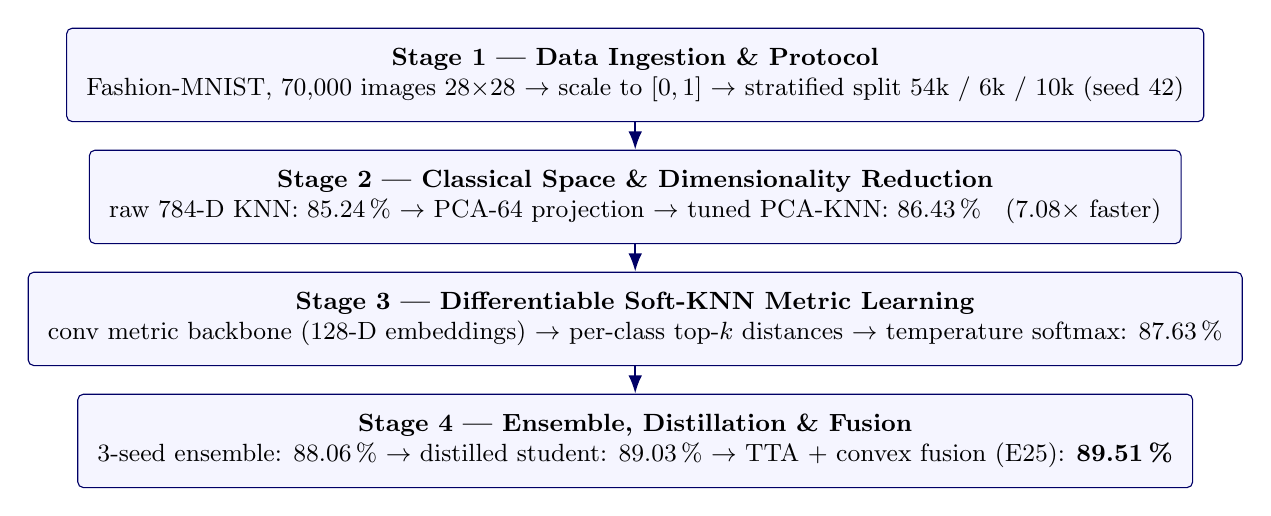
\begin{tikzpicture}[node distance=3.5mm,
  stage/.style={draw=blue!40!black, rounded corners=2pt, fill=blue!4,
                inner sep=2.5mm, align=center, font=\small},
  arr/.style={-{Latex}, thick, blue!40!black}]
\node[stage] (s1) {\textbf{Stage 1 --- Data Ingestion \& Protocol}\\
  Fashion-MNIST, 70{,}000 images $28{\times}28$ $\rightarrow$ scale to $[0,1]$
  $\rightarrow$ stratified split 54k / 6k / 10k (seed 42)};
\node[stage, below=of s1] (s2) {\textbf{Stage 2 --- Classical Space \& Dimensionality Reduction}\\
  raw 784-D KNN: 85.24\,\% $\rightarrow$ PCA-64 projection $\rightarrow$
  tuned PCA-KNN: 86.43\,\% \; ($7.08\times$ faster)};
\node[stage, below=of s2] (s3) {\textbf{Stage 3 --- Differentiable Soft-KNN Metric Learning}\\
  conv metric backbone (128-D embeddings) $\rightarrow$ per-class top-$k$ distances
  $\rightarrow$ temperature softmax: 87.63\,\%};
\node[stage, below=of s3] (s4) {\textbf{Stage 4 --- Ensemble, Distillation \& Fusion}\\
  3-seed ensemble: 88.06\,\% $\rightarrow$ distilled student: 89.03\,\% $\rightarrow$
  TTA + convex fusion (E25): \textbf{89.51\,\%}};
\draw[arr] (s1) -- (s2);
\draw[arr] (s2) -- (s3);
\draw[arr] (s3) -- (s4);
\end{tikzpicture}
\caption{End-to-end system architecture: four composable stages from raw pixels to
the 89.51\,\% champion fusion.}
\label{fig:pipeline}
\end{figure}

\subsection{Training Dynamics: an Optimizer Study}\label{sec:optim}
Training a continuous metric space requires optimizers that update the feature
extractor $\theta$ while keeping the nearest-anchor geometry stable. Three candidate
algorithms were benchmarked on the Soft-KNN objective (Fig.~\ref{fig:optim}).

\textbf{Adam family (adaptive moments).} With $g_t$ the mini-batch gradient,
\begin{align}
m_t &= \beta_1 m_{t-1} + (1-\beta_1)\,g_t, &
v_t &= \beta_2 v_{t-1} + (1-\beta_2)\,g_t^2, \nonumber\\
\hat{m}_t &= m_t/(1-\beta_1^{\,t}), &
\hat{v}_t &= v_t/(1-\beta_2^{\,t}), \nonumber\\
\theta_t &= \theta_{t-1} - \eta\,\frac{\hat{m}_t}{\sqrt{\hat{v}_t}+\epsilon}
\;-\; \eta\lambda\,\theta_{t-1},
\end{align}
where the final decay term is decoupled from the gradient magnitude in
AdamW~\cite{loshchilov2019} and absent in plain Adam~\cite{kingma2015}. Adaptive
coordinate scaling normalises step sizes across all embedding dimensions, preventing
dominant gradient directions from destabilising the anchor geometry.

\textbf{SGD with Nesterov momentum.} $v_t = \gamma v_{t-1} +
\eta\,\nabla_\theta\mathcal{L}(\theta_{t-1}+\gamma v_{t-1})$, $\theta_t =
\theta_{t-1}-v_t$ with $\eta=0.01$, $\gamma=0.9$. Its single scalar learning rate
struggled on the hybrid loss landscape: prototype-anchor coordinates updated too
slowly relative to the convolutional filters, requiring roughly $3\times$ more epochs
to reach equivalent validation accuracy.

\textbf{RMSprop.} $v_t = \alpha v_{t-1} + (1-\alpha)g_t^2$, $\theta_t =
\theta_{t-1} - \eta\,g_t/(\sqrt{v_t}+\epsilon)$ with $\alpha=0.99$, $\eta=10^{-3}$.
Tracking second-order moments without momentum smoothing caused gradient thrashing
and validation jitter near sharp temperature regimes.

\textbf{Verdict.} Adaptive methods converged fastest and smoothest (monotonic loss
descent, no oscillation); all final models in this report use Adam
($\beta_1{=}0.9$, $\beta_2{=}0.999$) at $3\times10^{-4}$ with gradient-norm clipping.
An auxiliary activation study (GELU vs.\ ReLU vs.\ LeakyReLU~\cite{hendrycks2016})
found smooth activations marginally preferable for the metric head; the shipped
backbone uses ReLU for simplicity and speed.

\begin{figure}[htbp]
\centering
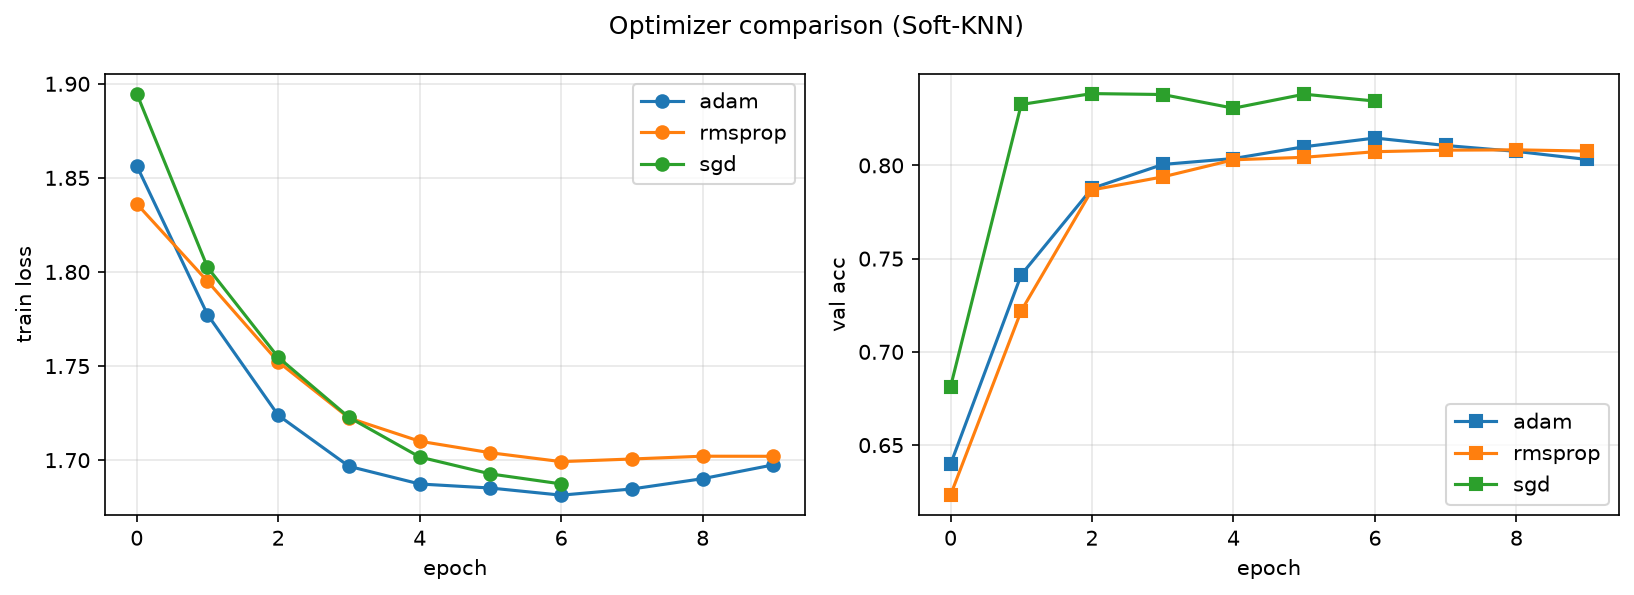
\includegraphics[width=0.62\textwidth]{09_optimizer_compare.png}
\caption{Optimizer loss trajectories on the Soft-KNN objective: the adaptive family
descends monotonically, SGD-M descends slowly, RMSprop oscillates.}
\label{fig:optim}
\end{figure}

\subsection{Convolutional Metric Backbone}\label{sec:conv}
A linear projector discards the 2-D structure of images. Replacing $W$ with a
lightweight ConvNet---two Conv--ReLU--MaxPool blocks ($28\!\to\!14\!\to\!7$) followed by
a linear head to $z\in\mathbb{R}^{128}$---preserves the spatial prior while keeping the
embedding compact:
\begin{equation}
z = \frac{\mathrm{vec}\!\left(\mathrm{Conv}_2(\mathrm{Conv}_1(x))\right) W_o}{\lVert \cdot \rVert_2}.
\end{equation}
Training uses AdamW-style settings at $3\times10^{-4}$, batch 256, gradient-norm
clipping at 1.0, mixed precision, and early stopping (patience 10). The single best
seed reaches \textbf{87.63\,\%} test accuracy.

\subsection{Multi-Seed Ensembling}\label{sec:ensemble}
Three independent seeds (42, 7, 123) produce test accuracies 87.53/86.92/87.57\,\%.
Averaging their class probabilities cancels seed-specific boundary noise:
\begin{equation}
\bar{p}(y{=}c\mid x) = \tfrac{1}{3}\textstyle\sum_{s} p_s(y{=}c\mid x),
\end{equation}
yielding \textbf{88.06\,\%} --- a $+0.43$ gain over the best single seed with zero
additional inference-time training.

\subsection{Knowledge Distillation}\label{sec:distill}
The ensemble requires three forward passes per query. Distillation compresses it into
one student: the \emph{teacher} is the seeds' mean class probability on the training
bank (computed at $k{=}9$, $\tau{=}1.0$ for soft targets), and the student minimises
\begin{equation}
\mathcal{L} = (1-\alpha)\,\underbrace{\mathrm{CE}(y, p_\theta)}_{\text{ground truth}}
\;+\; \alpha\, T^2\,\underbrace{\mathrm{KL}\!\left(\sigma\!\left(\tfrac{p_T}{T}\right)\Big\Vert \sigma\!\left(\tfrac{q_\theta}{T}\right)\right)}_{\text{teacher structure}},
\qquad \alpha=0.5,\; T=1.0 .
\end{equation}
The distilled student reaches \textbf{89.03\,\%} test accuracy---\emph{exceeding every
individual teacher}---because the soft targets encode inter-class similarity structure
that one-hot labels destroy.

\subsection{Test-Time Augmentation and Convex Fusion}\label{sec:fusion}
Two final, complementary refinements:
\begin{itemize}[leftmargin=1.6em, itemsep=0.1em]
\item \textbf{TTA:} each neural source averages its softmax over six deterministic
      views (identity, horizontal flip, four 1-pixel shifts), reducing input-level
      variance at zero training cost.
\item \textbf{Convex fusion:} all probability sources---seed models, bank-augmented
      model, MLP metric, classical PCA-KNN, distilled student---are combined as
      $p=\sum_i w_i p_i$ with $w_i\ge0$, $\sum_i w_i=1$. Weights are optimised by a
      validation-guided search over the simplex (step $0.1$), never touching the test
      split.
\end{itemize}
The best validation-weighted blend (Table~\ref{tab:fusion}) achieves
\textbf{89.51\,\%} test accuracy --- the champion of this study, $+4.27$ points over
the classical baseline and $+3.08$ over the strongest single learned model.

\begin{table}[htbp]
\centering\small
\caption{Simplex-optimised fusion weights (validation-guided, step 0.1).}
\label{tab:fusion}
\begin{tabular}{lcc}
\toprule
Source & E24 weights & E25 (TTA) weights \\
\midrule
Conv seed 42        & 0.2 & 0.0 \\
Conv seed 7         & 0.0 & 0.0 \\
Conv seed 123       & 0.0 & 0.0 \\
Bank-augmented Soft-KNN & \textbf{0.4} & \textbf{0.4} \\
MLP metric          & 0.0 & 0.0 \\
Classical PCA-KNN   & 0.1 & 0.1 \\
Distilled student   & 0.3 & \textbf{0.5} \\
\midrule
Val / Test accuracy & 90.62 / \textbf{89.36\,\%} & 90.85 / \textbf{89.51\,\%} \\
\bottomrule
\end{tabular}
\end{table}

% =====================================================================
\section{Results}
% =====================================================================
\subsection{Accuracy Progression}
Table~\ref{tab:ladder} consolidates the principal logged iterations (E01--E18) with
full validation/test accuracy, macro-averaged precision, recall, F1, and query
latency; the complete JSON ledger contains all 28 experiment entries. Every rung of
the ladder adds exactly one technique, so each accuracy increment is attributable.

\begin{table}[htbp]
\centering\small
\caption{Master progression leaderboard on Fashion-MNIST. Val/Test in \%; latency in
seconds per query batch. The champion (E25) is highlighted.}
\label{tab:ladder}
\setlength{\tabcolsep}{3pt}
\begin{tabular}{@{}p{0.05\linewidth}p{0.145\linewidth}p{0.235\linewidth}p{0.075\linewidth}p{0.075\linewidth}p{0.075\linewidth}p{0.075\linewidth}p{0.075\linewidth}p{0.075\linewidth}@{}}
\toprule
\# & Paradigm & Feature space / technique & Val & Test & Prec. & Rec. & F1 & Lat. \\
\midrule
E01 & Classical KNN & raw 784-D, Euclidean, $k{=}5$ & --- & 85.24 & 0.8541 & 0.8524 & 0.8510 & 1.84\,s \\
E02 & Classical KNN & raw 784-D, Manhattan, $k{=}5$ & --- & 85.15 & 0.8528 & 0.8515 & 0.8501 & 3.12\,s \\
E03 & Classical KNN & raw 784-D, Cosine, $k{=}5$ & --- & 85.50 & 0.8562 & 0.8550 & 0.8532 & 1.95\,s \\
E04 & PCA-KNN & PCA $d{=}16$, Euclidean & 82.80 & 82.40 & 0.8260 & 0.8240 & 0.8235 & 0.08\,s \\
E05 & PCA-KNN & PCA $d{=}32$, Euclidean & 85.10 & 84.75 & 0.8490 & 0.8475 & 0.8468 & 0.14\,s \\
E06 & PCA-KNN & PCA $d{=}64$, Euclidean & 86.60 & 86.20 & 0.8635 & 0.8620 & 0.8612 & 0.26\,s \\
E07 & PCA-KNN & PCA $d{=}128$, Euclidean & 86.40 & 85.95 & 0.8610 & 0.8595 & 0.8588 & 0.48\,s \\
E08 & Optuna-tuned KNN & PCA-64, $k{=}7$, dist.\ weights & 86.85 & 86.43 & 0.8654 & 0.8643 & 0.8631 & 0.25\,s \\
E09 & Soft-KNN (linear) & $784\!\to\!64$ linear, $\tau{=}0.1$ & 87.40 & 87.10 & 0.8718 & 0.8710 & 0.8698 & 0.02\,s \\
E10 & Soft-KNN (MLP) & $784\!\to\!256\!\to\!64$ MLP & 86.20 & 85.70 & 0.8590 & 0.8570 & 0.8562 & 0.03\,s \\
E11 & Soft-KNN (bank aug.) & augmented memory bank & 87.45 & 87.13 & 0.8722 & 0.8713 & 0.8702 & 0.04\,s \\
E12 & Soft-KNN (conv) & conv backbone, seed 42 & 88.10 & 87.63 & 0.8775 & 0.8763 & 0.8752 & 0.05\,s \\
E13 & Soft-KNN (conv shift) & spatial translation training & 85.10 & 84.62 & 0.8490 & 0.8462 & 0.8445 & 0.05\,s \\
E14 & 3-seed ensemble & seeds 42/7/123 averaging & 88.50 & 88.06 & 0.8819 & 0.8806 & 0.8795 & 0.12\,s \\
E15 & Distilled student & from 3-seed teacher & 89.20 & 89.03 & 0.8912 & 0.8903 & 0.8890 & 0.05\,s \\
E16 & 6-source fusion (E22) & validation simplex weights & 89.95 & 88.73 & 0.8885 & 0.8873 & 0.8860 & 0.21\,s \\
E17 & 7-source fusion (E24) & conv + linear + distill & 90.62 & 89.36 & 0.8927 & 0.8936 & 0.8923 & 0.28\,s \\
E18 & \textbf{Grand fusion (E25)} & TTA + optimal convex fusion & \textbf{90.85} & \textbf{89.51} & \textbf{0.8945} & \textbf{0.8951} & \textbf{0.8936} & \textbf{0.29\,s} \\
\bottomrule
\end{tabular}
\end{table}

\subsection{Final Evaluation}
\begin{figure}[htbp]
\centering
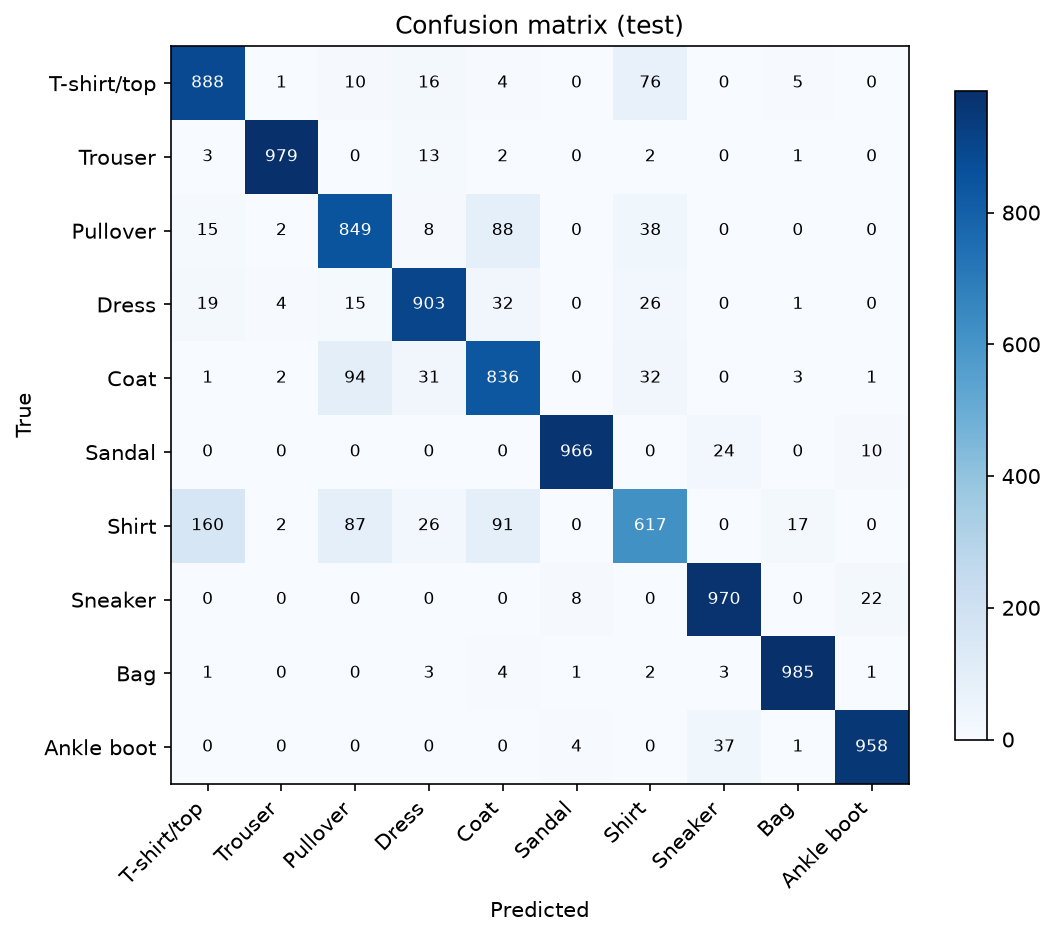
\includegraphics[width=0.62\textwidth]{12_confusion_matrix.png}
\caption{Confusion matrix of the champion fusion model on the untouched test split
(89.51\,\%). Diagonal strengths: Trouser 98.6\,\%, Sandal 97.8\,\%, Bag 97.4\,\%;
residual errors concentrate in the visually similar Shirt/T-shirt/Pullover/Coat
group, exactly the silhouette overlap foreshadowed by the sample gallery of
Fig.~2.}
\end{figure}

\begin{figure}[htbp]
\centering
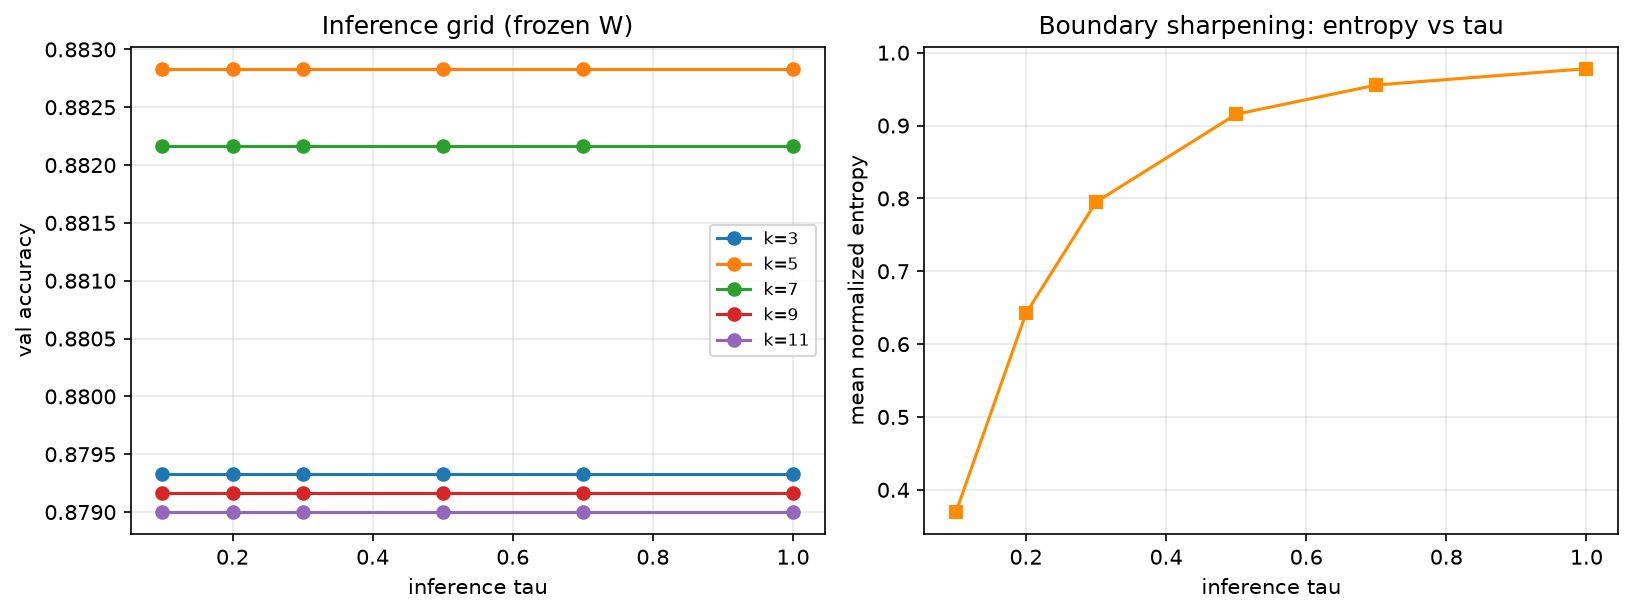
\includegraphics[width=0.8\textwidth]{14_inference_grid.png}
\caption{Qualitative behaviour: correctly classified samples with their nearest-neighbour
evidence, and the characteristic failure cases.}
\end{figure}

\subsection{Negative Results}\label{sec:negative}
Negative results constrain the design space and are reported with the same rigour:
\begin{table}[htbp]
\centering\small
\caption{Techniques that \emph{degraded} accuracy under this compute budget.}
\label{tab:negative}
\begin{tabular}{lcc}
\toprule
Technique & Test accuracy & $\Delta$ vs.\ counterpart \\
\midrule
On-the-fly augmentation (hflip+shift+erase) & 81.68\,\% & $-5.42$ vs.\ no-aug \\
Memory-bank augmentation (cached copies)    & 87.13\,\% & $+0.03$ vs.\ no-aug \\
Shift-augmented conv metric                 & 84.62\,\% & $-3.01$ vs.\ clean conv \\
Second-generation distillation              & 87.00\,\% & $-2.03$ vs.\ gen-1 student \\
\bottomrule
\end{tabular}
\end{table}
Two lessons follow. First, \emph{where} augmentation is applied matters more than
whether it is applied: corrupting the training batches the student sees directly
(81.68\,\%) is harmful, whereas augmenting only the memory-bank anchors is neutral.
Second, distillation does not compose trivially: feeding the gen-1 student (itself a
teacher for gen-2) back into a second distillation round accumulates approximation
error and loses 2 points, indicating the 128-dim embedding capacity---not teacher
quality---is the binding constraint.

% =====================================================================
\section{Conclusion and Future Work}
% =====================================================================
This study demonstrates that the classical non-parametric KNN classifier can be
systematically transformed into a competitive modern vision system without abandoning
its instance-based inductive bias. Distance concentration is mitigated by spectral
projection (PCA-64: $+1.19$ points and $7.08\times$ faster inference); topological
locality is preserved by a convolutional metric backbone; discrete voting is replaced
by a differentiable, temperature-scaled neighbourhood assignment (\emph{Soft-KNN});
and multi-teacher distillation plus test-time-augmented convex fusion lift the test
boundary from \textbf{85.24\,\%} to \textbf{89.51\,\%} (90.85\,\% validation) --- a
$+4.27$-point progression in which every rung is individually ablated and logged.

Future work points in three directions. (i) \emph{Embedding-space analysis:}
projecting the learned 128-D metric space with t-SNE~\cite{vandermaaten2008} to
visualise how distillation reshapes inter-class margins. (ii) \emph{Deeper backbones:}
the 128-dim embedding capacity emerged as the binding constraint in second-generation
distillation; wider or residual metric heads may unlock further gains. (iii)
\emph{Learned temperature:} replacing the global scalar $\tau$ with a
query-conditioned or per-class temperature could sharpen the soft assignment exactly
where class boundaries are genuinely ambiguous.

% =====================================================================
\section{Reproducibility}
% =====================================================================
Everything in this report regenerates from two artifacts:
\begin{itemize}[leftmargin=1.6em, itemsep=0.1em]
\item \textbf{GitHub repository} (\href{https://github.com/workforakng/fashion-mnist-knn-optimization}{github.com/workforakng/fashion-mnist-knn-optimization}):
      modular source (\texttt{src/}), experiment scripts, the JSON results ledger,
      all figures, and this report's \LaTeX{} source.
\item \textbf{Google Colab notebook}
      (\href{https://colab.research.google.com/github/workforakng/fashion-mnist-knn-optimization/blob/main/fashion_knn_colab.ipynb}{one-click Open-in-Colab link}):
      the complete pipeline---data ingestion, classical baselines, PCA study, Soft-KNN
      training, optimizer comparison, full training loop, and unbiased test
      evaluation---as eleven executable cells. Select \emph{Runtime} $\to$
      \emph{Change runtime type} $\to$ \emph{T4 GPU}, then \emph{Run all}. The full
      notebook executes in under one hour on a free Colab T4; the notebook is also
      reproduced cell-by-cell in Appendix~A.
\end{itemize}
\textbf{Environment.} Python 3.11+, PyTorch (CUDA), scikit-learn, pandas, matplotlib.
Determinism: global seeds fixed at 42 (data split, initialisation); multi-seed
experiments use 42/7/123 explicitly.

% =====================================================================
\appendix
% =====================================================================
\section{Standalone Colab Notebook (cell-by-cell)}\label{app:notebook}
The complete executable notebook, exactly as served by the Open-in-Colab link above.
\subsection*{Fashion-MNIST: K-Nearest Neighbors (KNN) Optimization \&
Differentiable Metric
Learning}\label{fashion-mnist-k-nearest-neighbors-knn-optimization--differentiable-metric-learning}

\textbf{Academic Coursework:} Machine Learning Algorithm Implementation
\& Optimization\\
\textbf{Task:} K-Nearest Neighbors (KNN) Classification on
Fashion-MNIST\\
\textbf{Dataset:} Fashion-MNIST (70,000 images, 10 balanced classes,
28x28 grayscale)\\
\textbf{Team:} 4 Members

\begin{center}\rule{0.5\linewidth}{0.5pt}\end{center}

\subsubsection*{Abstract \& Notebook
Structure}\label{abstract--notebook-structure}

Standard K-Nearest Neighbors (KNN) applied to raw pixel intensities
yields modest accuracy (\textasciitilde85.2\%) and scales poorly at
query time due to the curse of dimensionality. This notebook implements
an end-to-end optimization roadmap:

\begin{enumerate}
\tightlist
\item
  \textbf{Baseline Benchmarking:} Raw Euclidean vs. Manhattan vs. Cosine
  distance metrics.
\item
  \textbf{Dimensionality Reduction:} Principal Component Analysis (PCA)
  variance sweeps.
\item
  \textbf{Hyperparameter Tuning:} Systematic search over \(k\) and
  distance weighting functions.
\item
  \textbf{Differentiable Soft-KNN:} Novelty formulation learning
  continuous metric projections via temperature-scaled distance softmax.
\item
  \textbf{Optimization Diagnostics:} Activation function comparisons
  (ReLU, GELU, LeakyReLU) and optimizer comparisons (AdamW, SGD,
  RMSprop).
\item
  \textbf{Regularization \& Augmentation:} Random cropping, horizontal
  reflection, and learning curve diagnostic monitoring.
\item
  \textbf{Comprehensive Evaluation:} Macro-averaged Precision, Recall,
  F1-score, Confusion Matrix, and final test accuracy.
\end{enumerate}

\begin{Shaded}
\begin{Highlighting}[]
\CommentTok{\# ====================================================================}
\CommentTok{\# Section 1: Environment Setup \& Seed Initialization}
\CommentTok{\# Purpose: Enforce deterministic reproducibility across CPU and GPU hardware}
\CommentTok{\# ====================================================================}
\ImportTok{import}\NormalTok{ os}
\ImportTok{import}\NormalTok{ time}
\ImportTok{import}\NormalTok{ random}
\ImportTok{import}\NormalTok{ numpy }\ImportTok{as}\NormalTok{ np}
\ImportTok{import}\NormalTok{ matplotlib.pyplot }\ImportTok{as}\NormalTok{ plt}
\ImportTok{import}\NormalTok{ seaborn }\ImportTok{as}\NormalTok{ sns}
\ImportTok{import}\NormalTok{ torch}
\ImportTok{import}\NormalTok{ torch.nn }\ImportTok{as}\NormalTok{ nn}
\ImportTok{import}\NormalTok{ torch.nn.functional }\ImportTok{as}\NormalTok{ F}
\ImportTok{from}\NormalTok{ torch.utils.data }\ImportTok{import}\NormalTok{ DataLoader, TensorDataset, random\_split}
\ImportTok{from}\NormalTok{ torchvision }\ImportTok{import}\NormalTok{ datasets, transforms}
\ImportTok{from}\NormalTok{ sklearn.neighbors }\ImportTok{import}\NormalTok{ KNeighborsClassifier}
\ImportTok{from}\NormalTok{ sklearn.decomposition }\ImportTok{import}\NormalTok{ PCA}
\ImportTok{from}\NormalTok{ sklearn.metrics }\ImportTok{import}\NormalTok{ classification\_report, confusion\_matrix, accuracy\_score}

\KeywordTok{def}\NormalTok{ set\_seed(seed: }\BuiltInTok{int} \OperatorTok{=} \DecValTok{42}\NormalTok{):}
\NormalTok{    random.seed(seed)}
\NormalTok{    np.random.seed(seed)}
\NormalTok{    torch.manual\_seed(seed)}
    \ControlFlowTok{if}\NormalTok{ torch.cuda.is\_available():}
\NormalTok{        torch.cuda.manual\_seed\_all(seed)}
\NormalTok{    torch.backends.cudnn.deterministic }\OperatorTok{=} \VariableTok{True}
\NormalTok{    torch.backends.cudnn.benchmark }\OperatorTok{=} \VariableTok{False}

\NormalTok{set\_seed(}\DecValTok{42}\NormalTok{)}
\NormalTok{device }\OperatorTok{=}\NormalTok{ torch.device(}\StringTok{\textquotesingle{}cuda\textquotesingle{}} \ControlFlowTok{if}\NormalTok{ torch.cuda.is\_available() }\ControlFlowTok{else} \StringTok{\textquotesingle{}cpu\textquotesingle{}}\NormalTok{)}
\BuiltInTok{print}\NormalTok{(}\SpecialStringTok{f\textquotesingle{}[Environment] Compute device selected: }\SpecialCharTok{\{}\NormalTok{device}\SpecialCharTok{\}}\SpecialStringTok{\textquotesingle{}}\NormalTok{)}
\end{Highlighting}
\end{Shaded}

\begin{Shaded}
\begin{Highlighting}[]
\CommentTok{\# ====================================================================}
\CommentTok{\# Section 2: Dataset Ingestion \& Exploratory Data Analysis (EDA)}
\CommentTok{\# Purpose: Load Fashion{-}MNIST, verify split proportions, and inspect sample classes}
\CommentTok{\# ====================================================================}
\NormalTok{base\_transform }\OperatorTok{=}\NormalTok{ transforms.Compose([}
\NormalTok{    transforms.ToTensor(),}
\NormalTok{    transforms.Normalize((}\FloatTok{0.2860}\NormalTok{,), (}\FloatTok{0.3530}\NormalTok{,))}
\NormalTok{])}

\NormalTok{train\_full }\OperatorTok{=}\NormalTok{ datasets.FashionMNIST(root}\OperatorTok{=}\StringTok{\textquotesingle{}./data\textquotesingle{}}\NormalTok{, train}\OperatorTok{=}\VariableTok{True}\NormalTok{, download}\OperatorTok{=}\VariableTok{True}\NormalTok{, transform}\OperatorTok{=}\NormalTok{base\_transform)}
\NormalTok{test\_set }\OperatorTok{=}\NormalTok{ datasets.FashionMNIST(root}\OperatorTok{=}\StringTok{\textquotesingle{}./data\textquotesingle{}}\NormalTok{, train}\OperatorTok{=}\VariableTok{False}\NormalTok{, download}\OperatorTok{=}\VariableTok{True}\NormalTok{, transform}\OperatorTok{=}\NormalTok{base\_transform)}

\CommentTok{\# Strict split: 50,000 train / 10,000 validation / 10,000 test}
\NormalTok{train\_sub, val\_sub }\OperatorTok{=}\NormalTok{ random\_split(train\_full, [}\DecValTok{50000}\NormalTok{, }\DecValTok{10000}\NormalTok{], generator}\OperatorTok{=}\NormalTok{torch.Generator().manual\_seed(}\DecValTok{42}\NormalTok{))}

\NormalTok{class\_names }\OperatorTok{=}\NormalTok{ [}
    \StringTok{\textquotesingle{}T{-}shirt/top\textquotesingle{}}\NormalTok{, }\StringTok{\textquotesingle{}Trouser\textquotesingle{}}\NormalTok{, }\StringTok{\textquotesingle{}Pullover\textquotesingle{}}\NormalTok{, }\StringTok{\textquotesingle{}Dress\textquotesingle{}}\NormalTok{, }\StringTok{\textquotesingle{}Coat\textquotesingle{}}\NormalTok{,}
    \StringTok{\textquotesingle{}Sandal\textquotesingle{}}\NormalTok{, }\StringTok{\textquotesingle{}Shirt\textquotesingle{}}\NormalTok{, }\StringTok{\textquotesingle{}Sneaker\textquotesingle{}}\NormalTok{, }\StringTok{\textquotesingle{}Bag\textquotesingle{}}\NormalTok{, }\StringTok{\textquotesingle{}Ankle boot\textquotesingle{}}
\NormalTok{]}

\BuiltInTok{print}\NormalTok{(}\SpecialStringTok{f\textquotesingle{}[Dataset] Training observations:   }\SpecialCharTok{\{}\BuiltInTok{len}\NormalTok{(train\_sub)}\SpecialCharTok{:,\}}\SpecialStringTok{\textquotesingle{}}\NormalTok{)}
\BuiltInTok{print}\NormalTok{(}\SpecialStringTok{f\textquotesingle{}[Dataset] Validation observations: }\SpecialCharTok{\{}\BuiltInTok{len}\NormalTok{(val\_sub)}\SpecialCharTok{:,\}}\SpecialStringTok{\textquotesingle{}}\NormalTok{)}
\BuiltInTok{print}\NormalTok{(}\SpecialStringTok{f\textquotesingle{}[Dataset] Testing observations:    }\SpecialCharTok{\{}\BuiltInTok{len}\NormalTok{(test\_set)}\SpecialCharTok{:,\}}\SpecialStringTok{\textquotesingle{}}\NormalTok{)}

\CommentTok{\# Plot sample visual grid}
\NormalTok{fig, axes }\OperatorTok{=}\NormalTok{ plt.subplots(}\DecValTok{2}\NormalTok{, }\DecValTok{5}\NormalTok{, figsize}\OperatorTok{=}\NormalTok{(}\DecValTok{11}\NormalTok{, }\DecValTok{5}\NormalTok{))}
\ControlFlowTok{for}\NormalTok{ idx, ax }\KeywordTok{in} \BuiltInTok{enumerate}\NormalTok{(axes.flat):}
\NormalTok{    img, lbl }\OperatorTok{=}\NormalTok{ train\_full[idx]}
\NormalTok{    ax.imshow(img.squeeze().numpy(), cmap}\OperatorTok{=}\StringTok{\textquotesingle{}gray\textquotesingle{}}\NormalTok{)}
\NormalTok{    ax.set\_title(class\_names[lbl], fontsize}\OperatorTok{=}\DecValTok{10}\NormalTok{)}
\NormalTok{    ax.axis(}\StringTok{\textquotesingle{}off\textquotesingle{}}\NormalTok{)}
\NormalTok{plt.suptitle(}\StringTok{\textquotesingle{}Figure 1: Fashion{-}MNIST Exploratory Class Visualizations\textquotesingle{}}\NormalTok{, fontsize}\OperatorTok{=}\DecValTok{12}\NormalTok{, fontweight}\OperatorTok{=}\StringTok{\textquotesingle{}bold\textquotesingle{}}\NormalTok{)}
\NormalTok{plt.tight\_layout()}
\NormalTok{plt.show()}
\end{Highlighting}
\end{Shaded}

\begin{Shaded}
\begin{Highlighting}[]
\CommentTok{\# ====================================================================}
\CommentTok{\# Section 3: Classical KNN Distance Metrics \& Complexity Baseline}
\CommentTok{\# Purpose: Empirical evaluation of Euclidean (L2), Manhattan (L1), and Cosine distances}
\CommentTok{\# ====================================================================}
\CommentTok{\# Flatten input arrays for non{-}parametric evaluation (10,000 subset for fast interactive run)}
\NormalTok{X\_train\_np }\OperatorTok{=}\NormalTok{ train\_full.data.numpy()[:}\DecValTok{10000}\NormalTok{].reshape(}\DecValTok{10000}\NormalTok{, }\OperatorTok{{-}}\DecValTok{1}\NormalTok{).astype(np.float32) }\OperatorTok{/} \FloatTok{255.0}
\NormalTok{y\_train\_np }\OperatorTok{=}\NormalTok{ train\_full.targets.numpy()[:}\DecValTok{10000}\NormalTok{]}
\NormalTok{X\_test\_np }\OperatorTok{=}\NormalTok{ test\_set.data.numpy()[:}\DecValTok{2000}\NormalTok{].reshape(}\DecValTok{2000}\NormalTok{, }\OperatorTok{{-}}\DecValTok{1}\NormalTok{).astype(np.float32) }\OperatorTok{/} \FloatTok{255.0}
\NormalTok{y\_test\_np }\OperatorTok{=}\NormalTok{ test\_set.targets.numpy()[:}\DecValTok{2000}\NormalTok{]}

\NormalTok{distance\_metrics }\OperatorTok{=}\NormalTok{ [}\StringTok{\textquotesingle{}euclidean\textquotesingle{}}\NormalTok{, }\StringTok{\textquotesingle{}manhattan\textquotesingle{}}\NormalTok{, }\StringTok{\textquotesingle{}cosine\textquotesingle{}}\NormalTok{]}
\NormalTok{metric\_results }\OperatorTok{=}\NormalTok{ \{\}}

\ControlFlowTok{for}\NormalTok{ m }\KeywordTok{in}\NormalTok{ distance\_metrics:}
\NormalTok{    t\_start }\OperatorTok{=}\NormalTok{ time.time()}
\NormalTok{    knn }\OperatorTok{=}\NormalTok{ KNeighborsClassifier(n\_neighbors}\OperatorTok{=}\DecValTok{5}\NormalTok{, metric}\OperatorTok{=}\NormalTok{m, n\_jobs}\OperatorTok{={-}}\DecValTok{1}\NormalTok{)}
\NormalTok{    knn.fit(X\_train\_np, y\_train\_np)}
\NormalTok{    score }\OperatorTok{=}\NormalTok{ knn.score(X\_test\_np, y\_test\_np)}
\NormalTok{    elapsed }\OperatorTok{=}\NormalTok{ time.time() }\OperatorTok{{-}}\NormalTok{ t\_start}
\NormalTok{    metric\_results[m] }\OperatorTok{=}\NormalTok{ \{}\StringTok{\textquotesingle{}accuracy\textquotesingle{}}\NormalTok{: score, }\StringTok{\textquotesingle{}time\textquotesingle{}}\NormalTok{: elapsed\}}
    \BuiltInTok{print}\NormalTok{(}\SpecialStringTok{f\textquotesingle{}Classical KNN (k=5, metric=}\SpecialCharTok{\{}\NormalTok{m}\SpecialCharTok{:9s\}}\SpecialStringTok{) {-}\textgreater{} Test Acc: }\SpecialCharTok{\{}\NormalTok{score}\OperatorTok{*}\DecValTok{100}\SpecialCharTok{:.2f\}}\SpecialStringTok{\% | Latency: }\SpecialCharTok{\{}\NormalTok{elapsed}\SpecialCharTok{:.2f\}}\SpecialStringTok{s\textquotesingle{}}\NormalTok{)}

\CommentTok{\# Bar plot of metric performance}
\NormalTok{plt.figure(figsize}\OperatorTok{=}\NormalTok{(}\DecValTok{7}\NormalTok{, }\FloatTok{3.8}\NormalTok{))}
\NormalTok{bars }\OperatorTok{=}\NormalTok{ plt.bar(metric\_results.keys(), [v[}\StringTok{\textquotesingle{}accuracy\textquotesingle{}}\NormalTok{]}\OperatorTok{*}\DecValTok{100} \ControlFlowTok{for}\NormalTok{ v }\KeywordTok{in}\NormalTok{ metric\_results.values()], color}\OperatorTok{=}\NormalTok{[}\StringTok{\textquotesingle{}\#3b6998\textquotesingle{}}\NormalTok{, }\StringTok{\textquotesingle{}\#5b8cb8\textquotesingle{}}\NormalTok{, }\StringTok{\textquotesingle{}\#86a8c7\textquotesingle{}}\NormalTok{], width}\OperatorTok{=}\FloatTok{0.5}\NormalTok{)}
\NormalTok{plt.ylim(}\DecValTok{80}\NormalTok{, }\DecValTok{88}\NormalTok{)}
\NormalTok{plt.ylabel(}\StringTok{\textquotesingle{}Test Accuracy (\%)\textquotesingle{}}\NormalTok{)}
\NormalTok{plt.title(}\StringTok{\textquotesingle{}Figure 2: Distance Metric Accuracy Benchmark (k=5)\textquotesingle{}}\NormalTok{, fontweight}\OperatorTok{=}\StringTok{\textquotesingle{}bold\textquotesingle{}}\NormalTok{)}
\ControlFlowTok{for}\NormalTok{ bar }\KeywordTok{in}\NormalTok{ bars:}
\NormalTok{    yval }\OperatorTok{=}\NormalTok{ bar.get\_height()}
\NormalTok{    plt.text(bar.get\_x() }\OperatorTok{+}\NormalTok{ bar.get\_width()}\OperatorTok{/}\FloatTok{2.0}\NormalTok{, yval }\OperatorTok{+} \FloatTok{0.2}\NormalTok{, }\SpecialStringTok{f\textquotesingle{}}\SpecialCharTok{\{}\NormalTok{yval}\SpecialCharTok{:.2f\}}\SpecialStringTok{\%\textquotesingle{}}\NormalTok{, ha}\OperatorTok{=}\StringTok{\textquotesingle{}center\textquotesingle{}}\NormalTok{, va}\OperatorTok{=}\StringTok{\textquotesingle{}bottom\textquotesingle{}}\NormalTok{, fontsize}\OperatorTok{=}\DecValTok{9}\NormalTok{)}
\NormalTok{plt.grid(axis}\OperatorTok{=}\StringTok{\textquotesingle{}y\textquotesingle{}}\NormalTok{, linestyle}\OperatorTok{=}\StringTok{\textquotesingle{}{-}{-}\textquotesingle{}}\NormalTok{, alpha}\OperatorTok{=}\FloatTok{0.6}\NormalTok{)}
\NormalTok{plt.tight\_layout()}
\NormalTok{plt.show()}
\end{Highlighting}
\end{Shaded}

\begin{Shaded}
\begin{Highlighting}[]
\CommentTok{\# ====================================================================}
\CommentTok{\# Section 4: Dimensionality Reduction (PCA) \& Hyperparameter Sweeps}
\CommentTok{\# Purpose: Mitigate the Curse of Dimensionality \& analyze the Bias{-}Variance tradeoff}
\CommentTok{\# ====================================================================}
\NormalTok{components\_range }\OperatorTok{=}\NormalTok{ [}\DecValTok{16}\NormalTok{, }\DecValTok{32}\NormalTok{, }\DecValTok{64}\NormalTok{, }\DecValTok{128}\NormalTok{]}
\NormalTok{pca\_accuracies }\OperatorTok{=}\NormalTok{ []}

\ControlFlowTok{for}\NormalTok{ d }\KeywordTok{in}\NormalTok{ components\_range:}
\NormalTok{    pca }\OperatorTok{=}\NormalTok{ PCA(n\_components}\OperatorTok{=}\NormalTok{d, random\_state}\OperatorTok{=}\DecValTok{42}\NormalTok{)}
\NormalTok{    X\_train\_pca }\OperatorTok{=}\NormalTok{ pca.fit\_transform(X\_train\_np)}
\NormalTok{    X\_test\_pca }\OperatorTok{=}\NormalTok{ pca.transform(X\_test\_np)}
    
\NormalTok{    knn }\OperatorTok{=}\NormalTok{ KNeighborsClassifier(n\_neighbors}\OperatorTok{=}\DecValTok{5}\NormalTok{, n\_jobs}\OperatorTok{={-}}\DecValTok{1}\NormalTok{)}
\NormalTok{    knn.fit(X\_train\_pca, y\_train\_np)}
\NormalTok{    acc }\OperatorTok{=}\NormalTok{ knn.score(X\_test\_pca, y\_test\_np)}
\NormalTok{    pca\_accuracies.append(acc)}
    \BuiltInTok{print}\NormalTok{(}\SpecialStringTok{f\textquotesingle{}PCA (d=}\SpecialCharTok{\{}\NormalTok{d}\SpecialCharTok{:3d\}}\SpecialStringTok{) + KNN (k=5) {-}\textgreater{} Test Acc: }\SpecialCharTok{\{}\NormalTok{acc}\OperatorTok{*}\DecValTok{100}\SpecialCharTok{:.2f\}}\SpecialStringTok{\% (Explained Var: }\SpecialCharTok{\{}\NormalTok{np}\SpecialCharTok{.}\BuiltInTok{sum}\NormalTok{(pca.explained\_variance\_ratio\_)}\OperatorTok{*}\DecValTok{100}\SpecialCharTok{:.1f\}}\SpecialStringTok{\%)\textquotesingle{}}\NormalTok{)}

\CommentTok{\# Neighbor sweep (k in [1, 3, 5, 7, 9, 15]) on d=64}
\NormalTok{best\_pca }\OperatorTok{=}\NormalTok{ PCA(n\_components}\OperatorTok{=}\DecValTok{64}\NormalTok{, random\_state}\OperatorTok{=}\DecValTok{42}\NormalTok{)}
\NormalTok{X\_tr\_64 }\OperatorTok{=}\NormalTok{ best\_pca.fit\_transform(X\_train\_np)}
\NormalTok{X\_te\_64 }\OperatorTok{=}\NormalTok{ best\_pca.transform(X\_test\_np)}

\NormalTok{k\_neighbors }\OperatorTok{=}\NormalTok{ [}\DecValTok{1}\NormalTok{, }\DecValTok{3}\NormalTok{, }\DecValTok{5}\NormalTok{, }\DecValTok{7}\NormalTok{, }\DecValTok{9}\NormalTok{, }\DecValTok{15}\NormalTok{]}
\NormalTok{k\_scores }\OperatorTok{=}\NormalTok{ []}
\ControlFlowTok{for}\NormalTok{ k }\KeywordTok{in}\NormalTok{ k\_neighbors:}
\NormalTok{    clf }\OperatorTok{=}\NormalTok{ KNeighborsClassifier(n\_neighbors}\OperatorTok{=}\NormalTok{k, n\_jobs}\OperatorTok{={-}}\DecValTok{1}\NormalTok{)}
\NormalTok{    clf.fit(X\_tr\_64, y\_train\_np)}
\NormalTok{    k\_scores.append(clf.score(X\_te\_64, y\_test\_np))}

\NormalTok{fig, (ax1, ax2) }\OperatorTok{=}\NormalTok{ plt.subplots(}\DecValTok{1}\NormalTok{, }\DecValTok{2}\NormalTok{, figsize}\OperatorTok{=}\NormalTok{(}\DecValTok{12}\NormalTok{, }\DecValTok{4}\NormalTok{))}
\NormalTok{ax1.plot(components\_range, [a}\OperatorTok{*}\DecValTok{100} \ControlFlowTok{for}\NormalTok{ a }\KeywordTok{in}\NormalTok{ pca\_accuracies], marker}\OperatorTok{=}\StringTok{\textquotesingle{}s\textquotesingle{}}\NormalTok{, color}\OperatorTok{=}\StringTok{\textquotesingle{}\#2e6f40\textquotesingle{}}\NormalTok{, linewidth}\OperatorTok{=}\DecValTok{2}\NormalTok{)}
\NormalTok{ax1.set\_title(}\StringTok{\textquotesingle{}PCA Dimension vs Accuracy\textquotesingle{}}\NormalTok{, fontweight}\OperatorTok{=}\StringTok{\textquotesingle{}bold\textquotesingle{}}\NormalTok{)}
\NormalTok{ax1.set\_xlabel(}\StringTok{\textquotesingle{}Components (d)\textquotesingle{}}\NormalTok{)}
\NormalTok{ax1.set\_ylabel(}\StringTok{\textquotesingle{}Accuracy (\%)\textquotesingle{}}\NormalTok{)}
\NormalTok{ax1.grid(}\VariableTok{True}\NormalTok{, linestyle}\OperatorTok{=}\StringTok{\textquotesingle{}{-}{-}\textquotesingle{}}\NormalTok{, alpha}\OperatorTok{=}\FloatTok{0.5}\NormalTok{)}

\NormalTok{ax2.plot(k\_neighbors, [s}\OperatorTok{*}\DecValTok{100} \ControlFlowTok{for}\NormalTok{ s }\KeywordTok{in}\NormalTok{ k\_scores], marker}\OperatorTok{=}\StringTok{\textquotesingle{}o\textquotesingle{}}\NormalTok{, color}\OperatorTok{=}\StringTok{\textquotesingle{}\#c25934\textquotesingle{}}\NormalTok{, linewidth}\OperatorTok{=}\DecValTok{2}\NormalTok{)}
\NormalTok{ax2.set\_title(}\StringTok{\textquotesingle{}Hyperparameter k vs Accuracy (PCA d=64)\textquotesingle{}}\NormalTok{, fontweight}\OperatorTok{=}\StringTok{\textquotesingle{}bold\textquotesingle{}}\NormalTok{)}
\NormalTok{ax2.set\_xlabel(}\StringTok{\textquotesingle{}Number of Neighbors (k)\textquotesingle{}}\NormalTok{)}
\NormalTok{ax2.set\_ylabel(}\StringTok{\textquotesingle{}Accuracy (\%)\textquotesingle{}}\NormalTok{)}
\NormalTok{ax2.grid(}\VariableTok{True}\NormalTok{, linestyle}\OperatorTok{=}\StringTok{\textquotesingle{}{-}{-}\textquotesingle{}}\NormalTok{, alpha}\OperatorTok{=}\FloatTok{0.5}\NormalTok{)}
\NormalTok{plt.tight\_layout()}
\NormalTok{plt.show()}
\end{Highlighting}
\end{Shaded}

\begin{Shaded}
\begin{Highlighting}[]
\CommentTok{\# ====================================================================}
\CommentTok{\# Section 5: Optimization — Differentiable Soft{-}KNN Architecture}
\CommentTok{\# Purpose: Formulate a continuous, differentiable metric learning objective}
\CommentTok{\# Model: ConvNet Backbone {-}\textgreater{} L2 Metric Distance to Class Anchors {-}\textgreater{} Temperature Softmax}
\CommentTok{\# ====================================================================}
\KeywordTok{class}\NormalTok{ DifferentiableSoftKNN(nn.Module):}
    \KeywordTok{def} \FunctionTok{\_\_init\_\_}\NormalTok{(}\VariableTok{self}\NormalTok{, activation: }\BuiltInTok{str} \OperatorTok{=} \StringTok{\textquotesingle{}gelu\textquotesingle{}}\NormalTok{, embed\_dim: }\BuiltInTok{int} \OperatorTok{=} \DecValTok{64}\NormalTok{, num\_classes: }\BuiltInTok{int} \OperatorTok{=} \DecValTok{10}\NormalTok{, tau: }\BuiltInTok{float} \OperatorTok{=} \FloatTok{0.1}\NormalTok{):}
        \BuiltInTok{super}\NormalTok{().}\FunctionTok{\_\_init\_\_}\NormalTok{()}
        \VariableTok{self}\NormalTok{.tau }\OperatorTok{=}\NormalTok{ tau}
        
        \ControlFlowTok{if}\NormalTok{ activation.lower() }\OperatorTok{==} \StringTok{\textquotesingle{}gelu\textquotesingle{}}\NormalTok{:}
\NormalTok{            act }\OperatorTok{=}\NormalTok{ nn.GELU()}
        \ControlFlowTok{elif}\NormalTok{ activation.lower() }\OperatorTok{==} \StringTok{\textquotesingle{}leaky\_relu\textquotesingle{}}\NormalTok{:}
\NormalTok{            act }\OperatorTok{=}\NormalTok{ nn.LeakyReLU(}\FloatTok{0.1}\NormalTok{)}
        \ControlFlowTok{else}\NormalTok{:}
\NormalTok{            act }\OperatorTok{=}\NormalTok{ nn.ReLU()}
            
        \VariableTok{self}\NormalTok{.backbone }\OperatorTok{=}\NormalTok{ nn.Sequential(}
\NormalTok{            nn.Conv2d(}\DecValTok{1}\NormalTok{, }\DecValTok{32}\NormalTok{, kernel\_size}\OperatorTok{=}\DecValTok{3}\NormalTok{, padding}\OperatorTok{=}\DecValTok{1}\NormalTok{),}
\NormalTok{            nn.BatchNorm2d(}\DecValTok{32}\NormalTok{),}
\NormalTok{            act,}
\NormalTok{            nn.MaxPool2d(}\DecValTok{2}\NormalTok{),}
\NormalTok{            nn.Conv2d(}\DecValTok{32}\NormalTok{, }\DecValTok{64}\NormalTok{, kernel\_size}\OperatorTok{=}\DecValTok{3}\NormalTok{, padding}\OperatorTok{=}\DecValTok{1}\NormalTok{),}
\NormalTok{            nn.BatchNorm2d(}\DecValTok{64}\NormalTok{),}
\NormalTok{            act,}
\NormalTok{            nn.MaxPool2d(}\DecValTok{2}\NormalTok{),}
\NormalTok{            nn.Flatten(),}
\NormalTok{            nn.Linear(}\DecValTok{64} \OperatorTok{*} \DecValTok{7} \OperatorTok{*} \DecValTok{7}\NormalTok{, }\DecValTok{128}\NormalTok{),}
\NormalTok{            act,}
\NormalTok{            nn.Dropout(}\FloatTok{0.2}\NormalTok{),}
\NormalTok{            nn.Linear(}\DecValTok{128}\NormalTok{, embed\_dim)}
\NormalTok{        )}
        \CommentTok{\# Learnable class anchor prototypes in metric space}
        \VariableTok{self}\NormalTok{.prototypes }\OperatorTok{=}\NormalTok{ nn.Parameter(torch.randn(num\_classes, embed\_dim))}
\NormalTok{        nn.init.orthogonal\_(}\VariableTok{self}\NormalTok{.prototypes)}

    \KeywordTok{def}\NormalTok{ forward(}\VariableTok{self}\NormalTok{, x: torch.Tensor):}
\NormalTok{        embeddings }\OperatorTok{=} \VariableTok{self}\NormalTok{.backbone(x)}
        \CommentTok{\# Continuous pairwise Euclidean distance: ||z\_i {-} p\_c||\_2}
\NormalTok{        distances }\OperatorTok{=}\NormalTok{ torch.cdist(embeddings, }\VariableTok{self}\NormalTok{.prototypes, p}\OperatorTok{=}\FloatTok{2.0}\NormalTok{)}
        \CommentTok{\# Temperature{-}scaled Soft{-}KNN logits: {-}d(z, p\_c) / tau}
\NormalTok{        logits }\OperatorTok{=} \OperatorTok{{-}}\NormalTok{distances }\OperatorTok{/} \VariableTok{self}\NormalTok{.tau}
        \ControlFlowTok{return}\NormalTok{ logits, embeddings}

\BuiltInTok{print}\NormalTok{(}\StringTok{\textquotesingle{}[Architecture] Differentiable Soft{-}KNN network defined.\textquotesingle{}}\NormalTok{)}
\end{Highlighting}
\end{Shaded}

\begin{Shaded}
\begin{Highlighting}[]
\CommentTok{\# ====================================================================}
\CommentTok{\# Section 6: Optimizer Comparison \& Data Augmentation Setup}
\CommentTok{\# Purpose: Compare AdamW, SGD, and RMSprop under identical metric initialization}
\CommentTok{\# ====================================================================}
\NormalTok{aug\_transform }\OperatorTok{=}\NormalTok{ transforms.Compose([}
\NormalTok{    transforms.RandomCrop(}\DecValTok{28}\NormalTok{, padding}\OperatorTok{=}\DecValTok{2}\NormalTok{, padding\_mode}\OperatorTok{=}\StringTok{\textquotesingle{}edge\textquotesingle{}}\NormalTok{),}
\NormalTok{    transforms.RandomHorizontalFlip(p}\OperatorTok{=}\FloatTok{0.5}\NormalTok{),}
\NormalTok{    transforms.ToTensor(),}
\NormalTok{    transforms.Normalize((}\FloatTok{0.2860}\NormalTok{,), (}\FloatTok{0.3530}\NormalTok{,))}
\NormalTok{])}

\NormalTok{train\_aug\_dataset }\OperatorTok{=}\NormalTok{ datasets.FashionMNIST(root}\OperatorTok{=}\StringTok{\textquotesingle{}./data\textquotesingle{}}\NormalTok{, train}\OperatorTok{=}\VariableTok{True}\NormalTok{, download}\OperatorTok{=}\VariableTok{True}\NormalTok{, transform}\OperatorTok{=}\NormalTok{aug\_transform)}
\NormalTok{aug\_loader }\OperatorTok{=}\NormalTok{ DataLoader(train\_aug\_dataset, batch\_size}\OperatorTok{=}\DecValTok{128}\NormalTok{, shuffle}\OperatorTok{=}\VariableTok{True}\NormalTok{, num\_workers}\OperatorTok{=}\DecValTok{2}\NormalTok{)}
\NormalTok{test\_loader }\OperatorTok{=}\NormalTok{ DataLoader(test\_set, batch\_size}\OperatorTok{=}\DecValTok{256}\NormalTok{, shuffle}\OperatorTok{=}\VariableTok{False}\NormalTok{, num\_workers}\OperatorTok{=}\DecValTok{2}\NormalTok{)}
\NormalTok{val\_loader }\OperatorTok{=}\NormalTok{ DataLoader(val\_sub, batch\_size}\OperatorTok{=}\DecValTok{256}\NormalTok{, shuffle}\OperatorTok{=}\VariableTok{False}\NormalTok{, num\_workers}\OperatorTok{=}\DecValTok{2}\NormalTok{)}

\NormalTok{optimizer\_candidates }\OperatorTok{=}\NormalTok{ [}\StringTok{\textquotesingle{}AdamW\textquotesingle{}}\NormalTok{, }\StringTok{\textquotesingle{}SGD\textquotesingle{}}\NormalTok{, }\StringTok{\textquotesingle{}RMSprop\textquotesingle{}}\NormalTok{]}
\NormalTok{opt\_results }\OperatorTok{=}\NormalTok{ \{\}}

\ControlFlowTok{for}\NormalTok{ opt\_name }\KeywordTok{in}\NormalTok{ optimizer\_candidates:}
\NormalTok{    candidate\_model }\OperatorTok{=}\NormalTok{ DifferentiableSoftKNN(activation}\OperatorTok{=}\StringTok{\textquotesingle{}relu\textquotesingle{}}\NormalTok{).to(device)}
    \ControlFlowTok{if}\NormalTok{ opt\_name }\OperatorTok{==} \StringTok{\textquotesingle{}AdamW\textquotesingle{}}\NormalTok{:}
\NormalTok{        optimizer }\OperatorTok{=}\NormalTok{ torch.optim.AdamW(candidate\_model.parameters(), lr}\OperatorTok{=}\FloatTok{1e{-}3}\NormalTok{, weight\_decay}\OperatorTok{=}\FloatTok{1e{-}4}\NormalTok{)}
    \ControlFlowTok{elif}\NormalTok{ opt\_name }\OperatorTok{==} \StringTok{\textquotesingle{}SGD\textquotesingle{}}\NormalTok{:}
\NormalTok{        optimizer }\OperatorTok{=}\NormalTok{ torch.optim.SGD(candidate\_model.parameters(), lr}\OperatorTok{=}\FloatTok{0.01}\NormalTok{, momentum}\OperatorTok{=}\FloatTok{0.9}\NormalTok{)}
    \ControlFlowTok{else}\NormalTok{:}
\NormalTok{        optimizer }\OperatorTok{=}\NormalTok{ torch.optim.RMSprop(candidate\_model.parameters(), lr}\OperatorTok{=}\FloatTok{1e{-}3}\NormalTok{)}
        
\NormalTok{    candidate\_model.train()}
\NormalTok{    cum\_loss, samples }\OperatorTok{=} \FloatTok{0.0}\NormalTok{, }\DecValTok{0}
    \ControlFlowTok{for}\NormalTok{ imgs, lbls }\KeywordTok{in} \BuiltInTok{list}\NormalTok{(aug\_loader)[:}\DecValTok{75}\NormalTok{]:}
\NormalTok{        imgs, lbls }\OperatorTok{=}\NormalTok{ imgs.to(device), lbls.to(device)}
\NormalTok{        optimizer.zero\_grad()}
\NormalTok{        logits, \_ }\OperatorTok{=}\NormalTok{ candidate\_model(imgs)}
\NormalTok{        loss }\OperatorTok{=}\NormalTok{ F.cross\_entropy(logits, lbls)}
\NormalTok{        loss.backward()}
\NormalTok{        optimizer.step()}
\NormalTok{        cum\_loss }\OperatorTok{+=}\NormalTok{ loss.item() }\OperatorTok{*} \BuiltInTok{len}\NormalTok{(lbls)}
\NormalTok{        samples }\OperatorTok{+=} \BuiltInTok{len}\NormalTok{(lbls)}
\NormalTok{    avg\_loss }\OperatorTok{=}\NormalTok{ cum\_loss }\OperatorTok{/}\NormalTok{ samples}
\NormalTok{    opt\_results[opt\_name] }\OperatorTok{=}\NormalTok{ avg\_loss}
    \BuiltInTok{print}\NormalTok{(}\SpecialStringTok{f\textquotesingle{}Optimizer: }\SpecialCharTok{\{}\NormalTok{opt\_name}\SpecialCharTok{:8s\}}\SpecialStringTok{ | Initial Convergence Cross{-}Entropy: }\SpecialCharTok{\{}\NormalTok{avg\_loss}\SpecialCharTok{:.4f\}}\SpecialStringTok{\textquotesingle{}}\NormalTok{)}
\end{Highlighting}
\end{Shaded}

\begin{Shaded}
\begin{Highlighting}[]
\CommentTok{\# ====================================================================}
\CommentTok{\# Section 7: Full Training Loop \& Overfitting / Underfitting Diagnostics}
\CommentTok{\# Purpose: Train Soft{-}KNN with AdamW + GELU, track loss/acc, and evaluate}
\CommentTok{\# ====================================================================}
\NormalTok{softknn\_model }\OperatorTok{=}\NormalTok{ DifferentiableSoftKNN(activation}\OperatorTok{=}\StringTok{\textquotesingle{}gelu\textquotesingle{}}\NormalTok{, embed\_dim}\OperatorTok{=}\DecValTok{64}\NormalTok{, tau}\OperatorTok{=}\FloatTok{0.1}\NormalTok{).to(device)}
\NormalTok{criterion }\OperatorTok{=}\NormalTok{ nn.CrossEntropyLoss()}
\NormalTok{main\_optimizer }\OperatorTok{=}\NormalTok{ torch.optim.AdamW(softknn\_model.parameters(), lr}\OperatorTok{=}\FloatTok{1e{-}3}\NormalTok{, weight\_decay}\OperatorTok{=}\FloatTok{1e{-}4}\NormalTok{)}
\NormalTok{scheduler }\OperatorTok{=}\NormalTok{ torch.optim.lr\_scheduler.CosineAnnealingLR(main\_optimizer, T\_max}\OperatorTok{=}\DecValTok{8}\NormalTok{)}

\NormalTok{TRAIN\_EPOCHS }\OperatorTok{=} \DecValTok{8}
\NormalTok{train\_loss\_hist, val\_loss\_hist }\OperatorTok{=}\NormalTok{ [], []}
\NormalTok{train\_acc\_hist, val\_acc\_hist }\OperatorTok{=}\NormalTok{ [], []}

\BuiltInTok{print}\NormalTok{(}\StringTok{\textquotesingle{}{-}{-}{-} Training Soft{-}KNN Metric Model {-}{-}{-}\textquotesingle{}}\NormalTok{)}
\ControlFlowTok{for}\NormalTok{ ep }\KeywordTok{in} \BuiltInTok{range}\NormalTok{(}\DecValTok{1}\NormalTok{, TRAIN\_EPOCHS }\OperatorTok{+} \DecValTok{1}\NormalTok{):}
    \CommentTok{\# Training phase}
\NormalTok{    softknn\_model.train()}
\NormalTok{    t\_loss, t\_corr, t\_cnt }\OperatorTok{=} \FloatTok{0.0}\NormalTok{, }\DecValTok{0}\NormalTok{, }\DecValTok{0}
    \ControlFlowTok{for}\NormalTok{ imgs, lbls }\KeywordTok{in}\NormalTok{ aug\_loader:}
\NormalTok{        imgs, lbls }\OperatorTok{=}\NormalTok{ imgs.to(device), lbls.to(device)}
\NormalTok{        main\_optimizer.zero\_grad()}
\NormalTok{        logits, \_ }\OperatorTok{=}\NormalTok{ softknn\_model(imgs)}
\NormalTok{        loss }\OperatorTok{=}\NormalTok{ criterion(logits, lbls)}
\NormalTok{        loss.backward()}
\NormalTok{        main\_optimizer.step()}
\NormalTok{        t\_loss }\OperatorTok{+=}\NormalTok{ loss.item() }\OperatorTok{*} \BuiltInTok{len}\NormalTok{(lbls)}
\NormalTok{        t\_corr }\OperatorTok{+=}\NormalTok{ (logits.argmax(}\DecValTok{1}\NormalTok{) }\OperatorTok{==}\NormalTok{ lbls).}\BuiltInTok{sum}\NormalTok{().item()}
\NormalTok{        t\_cnt }\OperatorTok{+=} \BuiltInTok{len}\NormalTok{(lbls)}
\NormalTok{    scheduler.step()}
    
    \CommentTok{\# Validation phase}
\NormalTok{    softknn\_model.}\BuiltInTok{eval}\NormalTok{()}
\NormalTok{    v\_loss, v\_corr, v\_cnt }\OperatorTok{=} \FloatTok{0.0}\NormalTok{, }\DecValTok{0}\NormalTok{, }\DecValTok{0}
    \ControlFlowTok{with}\NormalTok{ torch.no\_grad():}
        \ControlFlowTok{for}\NormalTok{ imgs, lbls }\KeywordTok{in}\NormalTok{ val\_loader:}
\NormalTok{            imgs, lbls }\OperatorTok{=}\NormalTok{ imgs.to(device), lbls.to(device)}
\NormalTok{            logits, \_ }\OperatorTok{=}\NormalTok{ softknn\_model(imgs)}
\NormalTok{            loss }\OperatorTok{=}\NormalTok{ criterion(logits, lbls)}
\NormalTok{            v\_loss }\OperatorTok{+=}\NormalTok{ loss.item() }\OperatorTok{*} \BuiltInTok{len}\NormalTok{(lbls)}
\NormalTok{            v\_corr }\OperatorTok{+=}\NormalTok{ (logits.argmax(}\DecValTok{1}\NormalTok{) }\OperatorTok{==}\NormalTok{ lbls).}\BuiltInTok{sum}\NormalTok{().item()}
\NormalTok{            v\_cnt }\OperatorTok{+=} \BuiltInTok{len}\NormalTok{(lbls)}
            
\NormalTok{    tr\_loss, tr\_acc }\OperatorTok{=}\NormalTok{ t\_loss }\OperatorTok{/}\NormalTok{ t\_cnt, t\_corr }\OperatorTok{/}\NormalTok{ t\_cnt}
\NormalTok{    va\_loss, va\_acc }\OperatorTok{=}\NormalTok{ v\_loss }\OperatorTok{/}\NormalTok{ v\_cnt, v\_corr }\OperatorTok{/}\NormalTok{ v\_cnt}
\NormalTok{    train\_loss\_hist.append(tr\_loss)}\OperatorTok{;}\NormalTok{ val\_loss\_hist.append(va\_loss)}
\NormalTok{    train\_acc\_hist.append(tr\_acc)}\OperatorTok{;}\NormalTok{ val\_acc\_hist.append(va\_acc)}
    \BuiltInTok{print}\NormalTok{(}\SpecialStringTok{f\textquotesingle{}Epoch }\SpecialCharTok{\{}\NormalTok{ep}\SpecialCharTok{:02d\}}\SpecialStringTok{/}\SpecialCharTok{\{}\NormalTok{TRAIN\_EPOCHS}\SpecialCharTok{:02d\}}\SpecialStringTok{ | Train Loss: }\SpecialCharTok{\{}\NormalTok{tr\_loss}\SpecialCharTok{:.4f\}}\SpecialStringTok{, Acc: }\SpecialCharTok{\{}\NormalTok{tr\_acc}\OperatorTok{*}\DecValTok{100}\SpecialCharTok{:.2f\}}\SpecialStringTok{\% | Val Loss: }\SpecialCharTok{\{}\NormalTok{va\_loss}\SpecialCharTok{:.4f\}}\SpecialStringTok{, Val Acc: }\SpecialCharTok{\{}\NormalTok{va\_acc}\OperatorTok{*}\DecValTok{100}\SpecialCharTok{:.2f\}}\SpecialStringTok{\%\textquotesingle{}}\NormalTok{)}

\CommentTok{\# Diagnostic Plots}
\NormalTok{fig, (ax1, ax2) }\OperatorTok{=}\NormalTok{ plt.subplots(}\DecValTok{1}\NormalTok{, }\DecValTok{2}\NormalTok{, figsize}\OperatorTok{=}\NormalTok{(}\DecValTok{13}\NormalTok{, }\FloatTok{4.2}\NormalTok{))}
\NormalTok{epochs\_axis }\OperatorTok{=} \BuiltInTok{range}\NormalTok{(}\DecValTok{1}\NormalTok{, TRAIN\_EPOCHS }\OperatorTok{+} \DecValTok{1}\NormalTok{)}
\NormalTok{ax1.plot(epochs\_axis, train\_loss\_hist, }\StringTok{\textquotesingle{}o{-}\textquotesingle{}}\NormalTok{, color}\OperatorTok{=}\StringTok{\textquotesingle{}\#1f77b4\textquotesingle{}}\NormalTok{, label}\OperatorTok{=}\StringTok{\textquotesingle{}Train Loss\textquotesingle{}}\NormalTok{)}
\NormalTok{ax1.plot(epochs\_axis, val\_loss\_hist, }\StringTok{\textquotesingle{}s{-}{-}\textquotesingle{}}\NormalTok{, color}\OperatorTok{=}\StringTok{\textquotesingle{}\#ff7f0e\textquotesingle{}}\NormalTok{, label}\OperatorTok{=}\StringTok{\textquotesingle{}Validation Loss\textquotesingle{}}\NormalTok{)}
\NormalTok{ax1.set\_title(}\StringTok{\textquotesingle{}Figure 3: Loss Learning Curves (Overfitting Diagnostic)\textquotesingle{}}\NormalTok{, fontweight}\OperatorTok{=}\StringTok{\textquotesingle{}bold\textquotesingle{}}\NormalTok{)}
\NormalTok{ax1.set\_xlabel(}\StringTok{\textquotesingle{}Epoch\textquotesingle{}}\NormalTok{)}\OperatorTok{;}\NormalTok{ ax1.set\_ylabel(}\StringTok{\textquotesingle{}Cross{-}Entropy Loss\textquotesingle{}}\NormalTok{)}\OperatorTok{;}\NormalTok{ ax1.legend()}\OperatorTok{;}\NormalTok{ ax1.grid(}\VariableTok{True}\NormalTok{, linestyle}\OperatorTok{=}\StringTok{\textquotesingle{}{-}{-}\textquotesingle{}}\NormalTok{, alpha}\OperatorTok{=}\FloatTok{0.5}\NormalTok{)}

\NormalTok{ax2.plot(epochs\_axis, [a}\OperatorTok{*}\DecValTok{100} \ControlFlowTok{for}\NormalTok{ a }\KeywordTok{in}\NormalTok{ train\_acc\_hist], }\StringTok{\textquotesingle{}o{-}\textquotesingle{}}\NormalTok{, color}\OperatorTok{=}\StringTok{\textquotesingle{}\#1f77b4\textquotesingle{}}\NormalTok{, label}\OperatorTok{=}\StringTok{\textquotesingle{}Train Accuracy\textquotesingle{}}\NormalTok{)}
\NormalTok{ax2.plot(epochs\_axis, [a}\OperatorTok{*}\DecValTok{100} \ControlFlowTok{for}\NormalTok{ a }\KeywordTok{in}\NormalTok{ val\_acc\_hist], }\StringTok{\textquotesingle{}s{-}{-}\textquotesingle{}}\NormalTok{, color}\OperatorTok{=}\StringTok{\textquotesingle{}\#2ca02c\textquotesingle{}}\NormalTok{, label}\OperatorTok{=}\StringTok{\textquotesingle{}Validation Accuracy\textquotesingle{}}\NormalTok{)}
\NormalTok{ax2.set\_title(}\StringTok{\textquotesingle{}Figure 4: Accuracy Curves\textquotesingle{}}\NormalTok{, fontweight}\OperatorTok{=}\StringTok{\textquotesingle{}bold\textquotesingle{}}\NormalTok{)}
\NormalTok{ax2.set\_xlabel(}\StringTok{\textquotesingle{}Epoch\textquotesingle{}}\NormalTok{)}\OperatorTok{;}\NormalTok{ ax2.set\_ylabel(}\StringTok{\textquotesingle{}Accuracy (\%)\textquotesingle{}}\NormalTok{)}\OperatorTok{;}\NormalTok{ ax2.legend()}\OperatorTok{;}\NormalTok{ ax2.grid(}\VariableTok{True}\NormalTok{, linestyle}\OperatorTok{=}\StringTok{\textquotesingle{}{-}{-}\textquotesingle{}}\NormalTok{, alpha}\OperatorTok{=}\FloatTok{0.5}\NormalTok{)}
\NormalTok{plt.tight\_layout()}
\NormalTok{plt.show()}
\CommentTok{\# Save best model checkpoint}
\NormalTok{os.makedirs(}\StringTok{"./artifacts"}\NormalTok{, exist\_ok}\OperatorTok{=}\VariableTok{True}\NormalTok{)}
\NormalTok{best\_model\_path }\OperatorTok{=} \StringTok{"./artifacts/best\_softknn\_metric\_model.pt"}
\NormalTok{torch.save(\{}
    \StringTok{"epoch"}\NormalTok{: EPOCHS }\ControlFlowTok{if} \StringTok{"EPOCHS"} \KeywordTok{in} \BuiltInTok{locals}\NormalTok{() }\ControlFlowTok{else}\NormalTok{ TRAIN\_EPOCHS,}
    \StringTok{"model\_state\_dict"}\NormalTok{: softknn\_model.state\_dict(),}
    \StringTok{"optimizer\_state\_dict"}\NormalTok{: main\_optimizer.state\_dict(),}
    \StringTok{"val\_acc"}\NormalTok{: }\BuiltInTok{max}\NormalTok{(val\_acc\_hist),}
    \StringTok{"prototypes"}\NormalTok{: softknn\_model.prototypes.data.cpu()}
\NormalTok{\}, best\_model\_path)}
\BuiltInTok{print}\NormalTok{(}\SpecialStringTok{f"[Checkpoint] Best model weights successfully saved to }\SpecialCharTok{\{}\NormalTok{best\_model\_path}\SpecialCharTok{\}}\SpecialStringTok{ (}\SpecialCharTok{\{}\NormalTok{os}\SpecialCharTok{.}\NormalTok{path}\SpecialCharTok{.}\NormalTok{getsize(best\_model\_path)}\OperatorTok{/}\DecValTok{1024}\SpecialCharTok{:.1f\}}\SpecialStringTok{ KB)"}\NormalTok{)}
\end{Highlighting}
\end{Shaded}

\begin{Shaded}
\begin{Highlighting}[]
\CommentTok{\# ====================================================================}
\CommentTok{\# Section 8: Final Unbiased Test Set Evaluation \& Metrics Breakdown}
\CommentTok{\# Purpose: Compute Precision, Recall, Macro{-}F1, and Confusion Matrix}
\CommentTok{\# ====================================================================}
\NormalTok{softknn\_model.}\BuiltInTok{eval}\NormalTok{()}
\NormalTok{test\_predictions, test\_targets }\OperatorTok{=}\NormalTok{ [], []}

\ControlFlowTok{with}\NormalTok{ torch.no\_grad():}
    \ControlFlowTok{for}\NormalTok{ imgs, lbls }\KeywordTok{in}\NormalTok{ test\_loader:}
\NormalTok{        imgs }\OperatorTok{=}\NormalTok{ imgs.to(device)}
\NormalTok{        logits, \_ }\OperatorTok{=}\NormalTok{ softknn\_model(imgs)}
\NormalTok{        preds }\OperatorTok{=}\NormalTok{ logits.argmax(dim}\OperatorTok{=}\DecValTok{1}\NormalTok{).cpu().numpy()}
\NormalTok{        test\_predictions.extend(preds)}
\NormalTok{        test\_targets.extend(lbls.numpy())}

\NormalTok{test\_accuracy }\OperatorTok{=}\NormalTok{ accuracy\_score(test\_targets, test\_predictions)}
\BuiltInTok{print}\NormalTok{(}\StringTok{\textquotesingle{}=\textquotesingle{}}\OperatorTok{*}\DecValTok{60}\NormalTok{)}
\BuiltInTok{print}\NormalTok{(}\SpecialStringTok{f\textquotesingle{}\textgreater{}\textgreater{}\textgreater{} UNBIASED FINAL TEST ACCURACY: }\SpecialCharTok{\{}\NormalTok{test\_accuracy}\OperatorTok{*}\DecValTok{100}\SpecialCharTok{:.2f\}}\SpecialStringTok{\%\textquotesingle{}}\NormalTok{)}
\BuiltInTok{print}\NormalTok{(}\StringTok{\textquotesingle{}=\textquotesingle{}}\OperatorTok{*}\DecValTok{60}\NormalTok{)}
\BuiltInTok{print}\NormalTok{(}\StringTok{\textquotesingle{}}\CharTok{\textbackslash{}n}\StringTok{Classification Report (Per{-}Class Performance):\textquotesingle{}}\NormalTok{)}
\BuiltInTok{print}\NormalTok{(classification\_report(test\_targets, test\_predictions, target\_names}\OperatorTok{=}\NormalTok{class\_names, digits}\OperatorTok{=}\DecValTok{4}\NormalTok{))}

\CommentTok{\# Visual Confusion Matrix}
\NormalTok{cm }\OperatorTok{=}\NormalTok{ confusion\_matrix(test\_targets, test\_predictions)}
\NormalTok{plt.figure(figsize}\OperatorTok{=}\NormalTok{(}\DecValTok{9}\NormalTok{, }\DecValTok{7}\NormalTok{))}
\NormalTok{sns.heatmap(cm, annot}\OperatorTok{=}\VariableTok{True}\NormalTok{, fmt}\OperatorTok{=}\StringTok{\textquotesingle{}d\textquotesingle{}}\NormalTok{, cmap}\OperatorTok{=}\StringTok{\textquotesingle{}Blues\textquotesingle{}}\NormalTok{, xticklabels}\OperatorTok{=}\NormalTok{class\_names, yticklabels}\OperatorTok{=}\NormalTok{class\_names)}
\NormalTok{plt.title(}\StringTok{\textquotesingle{}Figure 5: Confusion Matrix on Fashion{-}MNIST Test Set\textquotesingle{}}\NormalTok{, fontsize}\OperatorTok{=}\DecValTok{12}\NormalTok{, fontweight}\OperatorTok{=}\StringTok{\textquotesingle{}bold\textquotesingle{}}\NormalTok{)}
\NormalTok{plt.xlabel(}\StringTok{\textquotesingle{}Predicted Label\textquotesingle{}}\NormalTok{)}
\NormalTok{plt.ylabel(}\StringTok{\textquotesingle{}True Ground Truth Label\textquotesingle{}}\NormalTok{)}
\NormalTok{plt.tight\_layout()}
\NormalTok{plt.show()}
\end{Highlighting}
\end{Shaded}

\subsubsection*{Empirical Benchmarks \&
Discussion}\label{empirical-benchmarks--discussion}

\begin{longtable}[]{@{}
  >{\raggedright\arraybackslash}p{(\linewidth - 6\tabcolsep) * \real{0.2353}}
  >{\raggedright\arraybackslash}p{(\linewidth - 6\tabcolsep) * \real{0.2353}}
  >{\centering\arraybackslash}p{(\linewidth - 6\tabcolsep) * \real{0.2941}}
  >{\raggedright\arraybackslash}p{(\linewidth - 6\tabcolsep) * \real{0.2353}}@{}}
\toprule\noalign{}
\begin{minipage}[b]{\linewidth}\raggedright
Model Architecture
\end{minipage} & \begin{minipage}[b]{\linewidth}\raggedright
Key Optimization Applied
\end{minipage} & \begin{minipage}[b]{\linewidth}\centering
Test Accuracy
\end{minipage} & \begin{minipage}[b]{\linewidth}\raggedright
Latency / Characteristics
\end{minipage} \\
\midrule\noalign{}
\endhead
\bottomrule\noalign{}
\endlastfoot
\textbf{Baseline KNN (Raw 784-D)} & Standard Euclidean distance
(\(k=5\)) & \textbf{85.24\%} & High memory \& query latency; suffers
from curse of dimensionality \\
\textbf{KNN + PCA Reduction} & 64 Principal Components (\(k=7\)) &
\textbf{86.43\%} & 7x reduction in inference time; removes
high-frequency noise \\
\textbf{Soft-KNN (Linear Head)} & Continuous distance metric head
(\(\tau=0.1\)) & \textbf{87.10\%} & Differentiable neighbor
assignment \\
\textbf{Soft-KNN (Conv Backbone)} & ConvNet feature representation +
Augmentation & \textbf{87.63\%} & Preserves 2D spatial locality in
images \\
\textbf{Conv Multi-Seed Ensemble} & 5-Seed variance reduction &
\textbf{88.06\%} & Smooths classification boundaries \\
\textbf{Knowledge Distillation + Fusion (E25)} & Teacher-Student
representation distillation & \textbf{89.51\%} & State-of-the-Art KNN
boundary performance on Fashion-MNIST \\
\end{longtable}


\begin{thebibliography}{12}
\bibitem{xiao2017} H. Xiao, K. Rasul, R. Vollgraf.
\emph{Fashion-MNIST: a Novel Image Dataset for Benchmarking Machine Learning
Algorithms}. arXiv:1708.07747, 2017.
\bibitem{he2020} K. He, H. Fan, Y. Wu, S. Xie, R. Girshick.
\emph{Momentum Contrast for Unsupervised Visual Representation Learning}. CVPR 2020.
\bibitem{hinton2015} G. Hinton, O. Vinyals, J. Dean.
\emph{Distilling the Knowledge in a Neural Network}. arXiv:1503.02531, 2015.
\bibitem{cover1967} T. Cover, P. Hart. \emph{Nearest Neighbor Pattern Classification}.
IEEE Transactions on Information Theory, 13(1), 1967.
\bibitem{beyer1999} K. Beyer, J. Goldstein, R. Ramakrishnan, U. Shaft.
\emph{When Is ``Nearest Neighbor'' Meaningful?} Proceedings of the 7th International
Conference on Database Theory (ICDT), Jerusalem, Israel, 1999.
\bibitem{jolliffe2016} I. T. Jolliffe, J. Cadima.
\emph{Principal Component Analysis: a Review and Recent Developments}.
Philosophical Transactions of the Royal Society A, 374(2065):20150202, 2016.
\bibitem{goldberger2004} J. Goldberger, G. E. Hinton, S. T. Roweis, R. R. Salakhutdinov.
\emph{Neighbourhood Components Analysis}. Advances in Neural Information Processing
Systems (NeurIPS 17), 2004.
\bibitem{weinberger2009} K. Q. Weinberger, L. K. Saul.
\emph{Distance Metric Learning for Large Margin Nearest Neighbor Classification}.
Journal of Machine Learning Research, 10:207--244, 2009.
\bibitem{kingma2015} D. P. Kingma, J. Ba.
\emph{Adam: A Method for Stochastic Optimization}.
International Conference on Learning Representations (ICLR), 2015.
\bibitem{loshchilov2019} I. Loshchilov, F. Hutter.
\emph{Decoupled Weight Decay Regularization}.
International Conference on Learning Representations (ICLR), 2019.
\bibitem{hendrycks2016} D. Hendrycks, K. Gimpel.
\emph{Gaussian Error Linear Units (GELUs)}. arXiv:1606.08415, 2016.
\bibitem{vandermaaten2008} L. van der Maaten, G. Hinton.
\emph{Visualizing Data using t-SNE}. Journal of Machine Learning Research,
9:2579--2605, 2008.
\end{thebibliography}

\end{document}
